% !TEX root =  thesis.tex
\documentclass[11pt,oneside,a4paper]{book}
\usepackage[latin1]{inputenc}
\usepackage{amsmath}
\usepackage{amssymb}
%f�r das Einbinden von Bildern und Tabellen
\usepackage{booktabs} 		%f�r tolle tabellen
\usepackage{threeparttable}
\usepackage{longtable}
%\usepackage[normal,small,bf]{caption} %erm�glicht mehrzeilige Bildunterschriften use [hang] f�r einger�ckte Bildunterschrift


\usepackage{psfrag}
%f�r die Bibliography
\usepackage{natbib}		% more flexibility with citations
\usepackage{ifpdf}
\usepackage{footnote}
%Verwendung von Farben
\usepackage{xcolor}
%bedruckten Bereich der Seite anpassen
\usepackage[left=3.0cm, right=2.5cm, top=2.5cm,bottom=2.0cm,includeheadfoot]{geometry}
% Formatierung Kapitelueberschriften
\usepackage{titlesec}
\usepackage[T1]{fontenc} % sonst geht \hyphenation nicht mit Umlauten
\usepackage{listings}
\usepackage{color}
\usepackage{wrapfig}
\usepackage{tikz}
\newcommand*\circled[1]{\tikz[baseline=(char.base)]{
            \node[shape=circle,draw,inner sep=1pt] (char) {#1};}}
 
\usepackage{lmodern}

\lstset{ %
  language=Java,                % the language of the code
  basicstyle=\ttfamily\footnotesize,           % the size of the fonts that are used for the code
  numbers=left,                   % where to put the line-numbers
  numberstyle=\tiny\color{gray},  % the style that is used for the line-numbers
  stepnumber=2,                   % the step between two line-numbers. If it's 1, each line 
                                  % will be numbered
  numbersep=5pt,                  % how far the line-numbers are from the code
  backgroundcolor=\color{white},      % choose the background color. You must add \usepackage{color}
  showspaces=false,               % show spaces adding particular underscores
  showstringspaces=false,         % underline spaces within strings
  showtabs=false,                 % show tabs within strings adding particular underscores
  frame=shadowbox,                   % adds a frame around the code
  rulecolor=\color{gray},        % if not set, the frame-color may be changed on line-breaks within not-black text (e.g. commens (green here))
  tabsize=2,                      % sets default tabsize to 2 spaces
  captionpos=b,                   % sets the caption-position to bottom
  breaklines=true,                % sets automatic line breaking
  breakatwhitespace=false,        % sets if automatic breaks should only happen at whitespace
  title=\lstname,                   % show the filename of files included with \lstinputlisting;
                                  % also try caption instead of title
  keywordstyle=\color{black},          % keyword style
  commentstyle=\color{black},       % comment style
  stringstyle=\color{black},         % string literal style
  escapeinside={\%*}{*)},            % if you want to add LaTeX within your code
  morekeywords={*,...}               % if you want to add more keywords to the set
}



%\titleformat{?�berschriftenklasse?}[Absatzformatierung?]{?Textformatierung?} {?Nummerierung?}{?Abstand zwischen Nummerierung und �berschriftentext?}{?Code vor der �berschrift?}[?Code nach der �berschrift?]
%\titleformat{\chapter}[hang]{\huge\bfseries}{\thechapter\quad}{0pt}{}
%\titlespacing{?�berschriftenklasse?}{?Linker Einzug?}{?Platz oberhalb?}{?Platz unterhalb?}[?rechter Einzug?]
%\titlespacing{\chapter}{0pt}{0em}{6pt}
%----------------------------------------------------------------------------------------------------------------------------------------------
%Stil der Seite
\usepackage{fancyhdr}
\fancypagestyle{plain}{%
	\fancyhf{} % clear all header and footer fields
	\fancyhead[EL,OR]{\slshape \thepage} % except the center
	\fancyhead[ER]{\slshape \leftmark}
	\fancyhead[OL]{\slshape \rightmark}
}
\renewcommand{\chaptermark}[1]{\markboth{\thechapter. #1}{}}
\renewcommand{\sectionmark}[1]{\markright{\thesection. #1}{}}
%
\pagestyle{empty}%f�r die Titelseiten zumindest, am Ende der Titelseite umschalten auf \pagestyle{fancyplain}
\pagenumbering{Roman}%f�r die Titelseiten zumindest, am Ende der Titelseite umschalten auf \pagenumbering{arabic}
%------------------------je nach Kommando (pdflatex / latex) jeweilige Paketeinbindung-----------------------------
\definecolor{linkblue}{rgb}{0,0.1,0.6}
\definecolor{citegreen}{rgb}{0,0.25,0.15}%{0.1,0.5,0.4}%{0.125,0.6,0.5}
\definecolor{linkred}{rgb}{0.8,0,0.005}%{0.6,0,0.1}
\definecolor{mailviolet}{rgb}{0.3,0,0.35}%{0.6,0,0.1}
\definecolor{tumblue}{rgb}{0,0.396,0.741}

% Zum Setzen von URLs
\definecolor{darkred}{rgb}{.25,0,0}
\definecolor{darkgreen}{rgb}{0,.2,0}
\definecolor{darkmagenta}{rgb}{.2,0,.2}
\definecolor{darkcyan}{rgb}{0,.15,.15}
\usepackage[plainpages=false,bookmarks=true,bookmarksopen=true,colorlinks=true,
  linkcolor=darkred,citecolor=darkgreen,filecolor=darkmagenta,
  menucolor=darkred,urlcolor=darkcyan]{hyperref}


% pdflatex: Bilder in den Formaten .jpeg, .png und .pdf
% latex: Bilder im .eps-Format
\usepackage{graphicx}

\usepackage[ngerman]{babel}
\usepackage[latin1]{inputenc}
\usepackage[T1]{fontenc}

%Zeilenabst�nde regulieren mit \singlespacing, \onehalfspacing, \doublespacing
\usepackage{subfig} %{subfigure} alt
\usepackage{setspace}
\onehalfspacing
\parindent 0pt
%Schriftart Sans Serif
%\renewcommand*\familydefault{\sfdefault} 




%mit allen noetigen Stildefinitionen, Paketeinbindungen, etc. - FIX
%---------------------------------- Bitte ausfuellen! --------------------------------
\newcommand{\DAtype}{Bachelorarbeit\\[1ex] 
}%Experimentelle/Theoretische/Konstruktive Semesterarbeit/Diplomarbeit
\newcommand{\DAthema}{Webbasierte 3D-Postvisualisierung \\ von Fu�g�ngersimulationsdaten}
\newcommand{\DAautor}{Daniel B�chele}
\newcommand{\Matrikel}{10022975 (LMU)}
\newcommand{\DAort}{M�nchen}%f�r Unterschrift, Ort, Datum
\newcommand{\DAautorAnschrift}{Clermontstr.~10\\D-82131 Gauting\\e-Mail: daniel@buechele.cc}
\newcommand{\DAprofessor}{Dipl.-Inf. Angelika Kneidl} %1. und offizieller 
\newcommand{\DAbetreuer}{Mustafa K. Isik} %2. und i.d.R. inoffizieller Betreuer
\newcommand{\DAausgabe}{30. April 2012}
\newcommand{\DAabgabe}{17. September 2012}
\newcommand{\AdresseLehrstuhl}{Fakult�t f�r Bauingenieur- und Vermessungswesen\\
Lehrstuhl f�r Computergest�tzte Modellierung und Simulation\\
Technische Universit�t M�nchen\\
Arcisstra�e 21\\
D-80333 M�nchen}
%--------------------------------------------------------------------------------------------


\hyphenation{Java-Script}
\hyphenation{WebGL}


\begin{document}
% !TEX root =  thesis.tex
%-------------------------------Kopf----------------------------------
\ \\[-1cm]

\includegraphics[height=1.5cm]{pictures/Logos/bauiverm.pdf}
\rule{5mm}{0pt}
\hfill

\includegraphics[height=1.5cm]{pictures/Logos/TUMLogo.pdf}
%\includegraphics{../pictures/Logos/TUMLogo_oZ_Outline_blau_RGB}
\\[0.75cm]
{\large Fakult�t f�r Bauingenieur- und Vermessungswesen\\[0.5ex]
Lehrstuhl f�r Computergest�tzte Modellierung und Simulation \\
Prof. Dr.-Ing. Andr� Borrmann}
\ \\[11ex]
%---------------------------------Thema und Autor--------------------------------
%%%%%%%%%%%%%%
\begin{spacing}{2.0}
	{\color{tumblue}{\huge{\bf{\DAthema}}}}
\end{spacing}
\ \\[5ex]
{\Large{\bf{\DAautor}}}\\[5ex]
{\Large{{\DAtype}}}\\[5ex]
\ \\
\vfill
%-----------------------------weitere Angaben -----------------------------------
\begin{tabbing}
Lehrstuhlinhaber: xxxx   \= \DAprofessor \kill %zur Abstandsdefinition
Autor:      \> \DAautor \\[1ex]
Matrikelnummer: \> \Matrikel \\[1ex]
BetreuerIn:       \> \DAprofessor \\[1ex]
                \> \DAbetreuer\\[1ex]
Anmeldedatum:   \> \DAausgabe \\[1ex]
Abgabedatum:    \> \DAabgabe
\end{tabbing}
%-----------------------
\cleardoublepage
		% FIX, titelseite.tex braucht i.d.R. nicht modifiziert zu werden!
%-------------------------------Kopf----------------------------------
\ \\[-1cm]

\includegraphics[height=1.5cm]{./pictures/Logos/bauiverm.pdf}
\rule{5mm}{0pt}
\hfill

\includegraphics[height=1.5cm]{./pictures/Logos/TUMLogo.pdf}
\\
\ \\[4ex]
%------------------------- Beteiligte Organisationen -----------------
\singlespacing\noindent%%%%%%%%%%%%%%%
{\color{tumblue}{\huge\bf{Beteiligte Organisationen}}}\\[5ex]
\parbox[c]{13.5cm}{\AdresseLehrstuhl}
\\[5ex]

Ludwig-Maximilians-Universit�t M�nchen \\
Institut f�r Informatik \\
LFE Medieninformatik \\
Amalienstra�e 17 \\
Vordergeb�ude, 5. Stock, Zimmer 507 \\
D-80333 M�nchen
\\[10ex]
%------------------------- Eidesstattliche Erkl�rung -----------------
{\color{tumblue}{\huge\bf{Selbstst�ndigkeitserkl�rung}}}\\[5ex]
Ich erkl�re hiermit, dass ich die vorliegende Arbeit selbstst�ndig angefertigt, alle Zitate als solche kenntlich gemacht sowie alle benutzten Quellen und Hilfsmittel angegeben habe. Diese Arbeit wurde zuvor nicht bei einer anderen akademischen Institution eingereicht oder anderweitig ver�ffentlicht. \\[3ex]
\DAort, \today\\[-4ex]
\begin{flushright}{\rule{7cm}{0.5pt}}\\{\footnotesize{\DAautor}}\end{flushright}
\ \\\vfill\noindent
\DAautor\\
\DAautorAnschrift
\cleardoublepage
		% falls es sich um eine Diplomarbeit handelt, hier eidesstattliche Erklaerung einbinden; auch FIX und nicht abzuaendern, bei Semesterarbeiten ist mit dem Betreuer abzuklaeren ob diese noetig ist.
\tableofcontents		% Inhaltsverzeichnix
\cleardoublepage
%--------------------------- Ab hier der eigentliche Inhalt der SA ---------------------
\pagestyle{plain}		% fancy header
\parskip 8pt
%\renewcommand{\chaptermark}[1]{\markboth{\thechapter. #1}{}}
%\renewcommand{\sectionmark}[1]{\markright{\thesection. #1}{}}
\pagenumbering{arabic}




%\input{chapter/01_Introduction}
%\input{chapter/02_Theory}
%\input{chapter/03_Conclusion}

\include{chapter/einleitung}

\section{Moderne Webtechnologien}

Das \emph{World Wide Web Consortium (W3C)} standardisiert Technologien die das Internet betreffen. Das Konsortium besteht aus �ber 300 Mitgliedern\footnote{Stand: August 2012} \ref{w3cmembers}, die �ber die Entstehung neuer Standards beraten und entscheiden. Da die Entstehung und Ver�ffentlichung neuer Standards beim W3C auf Grund der hohen Mitgliederzahl und demokratischen Strukturen oft sehr lange dauert, gr�ndeten Vertreter von Opera, Apple und Mozilla die \emph{Web Hypertext Application Technology Working Group (WHATWG)}. Eine Arbeitsgruppe, deren Mitgliedschaft nur auf Einladung erfolgt und deren endg�ltige Entscheidungen einem Vorsitzenden unterliegen. Erarbeitete Entw�rfe reicht die WHATWG beim W3C als Vorschlag zur Standardisierung ein. Einen Vorschlag der WHATWG nahm das W3C auch als Basis f�r die Spezifizierung von \emph{HTML5}. \ref{aboutw3c} \ref{keith}

\subsection{Der HTML5-Standard}
In der Spezifikation des W3C wird mit ``HTML5'' die Weiterentwicklung der Auszeichnungssprache HTML beschrieben. Die WHATWG dehnt den Begriff etwas weiter aus und versammelt unter dieser Bezeichnung auch einige JavaScript-Schnittstellen, wie etwa f�r das canvas-Element (siehe Kapitel \ref{canvasapi}), das \emph{WebSockets}-Netzwerkprotokoll oder die Nutzung von lokalem Speicher (\emph{WebStorage}). Im Sprachgebrauch wird der Begriff ``HTML5'' oft noch weiter gefasst und beinhaltet diverse weitere Technologien, die im Zuge moderner Web-Applikationen entwickelt wurden. Darunter fallen dann die Grafikbibliothek \emph{WebGL}, die \emph{Geo-Location}-API zur Abfrage des Standorts oder auch der \emph{CSS3}-Standard zur Gestaltung von Webseiten. (siehe Abbildung \ref{specgraphfig})

\begin{figure}[h]
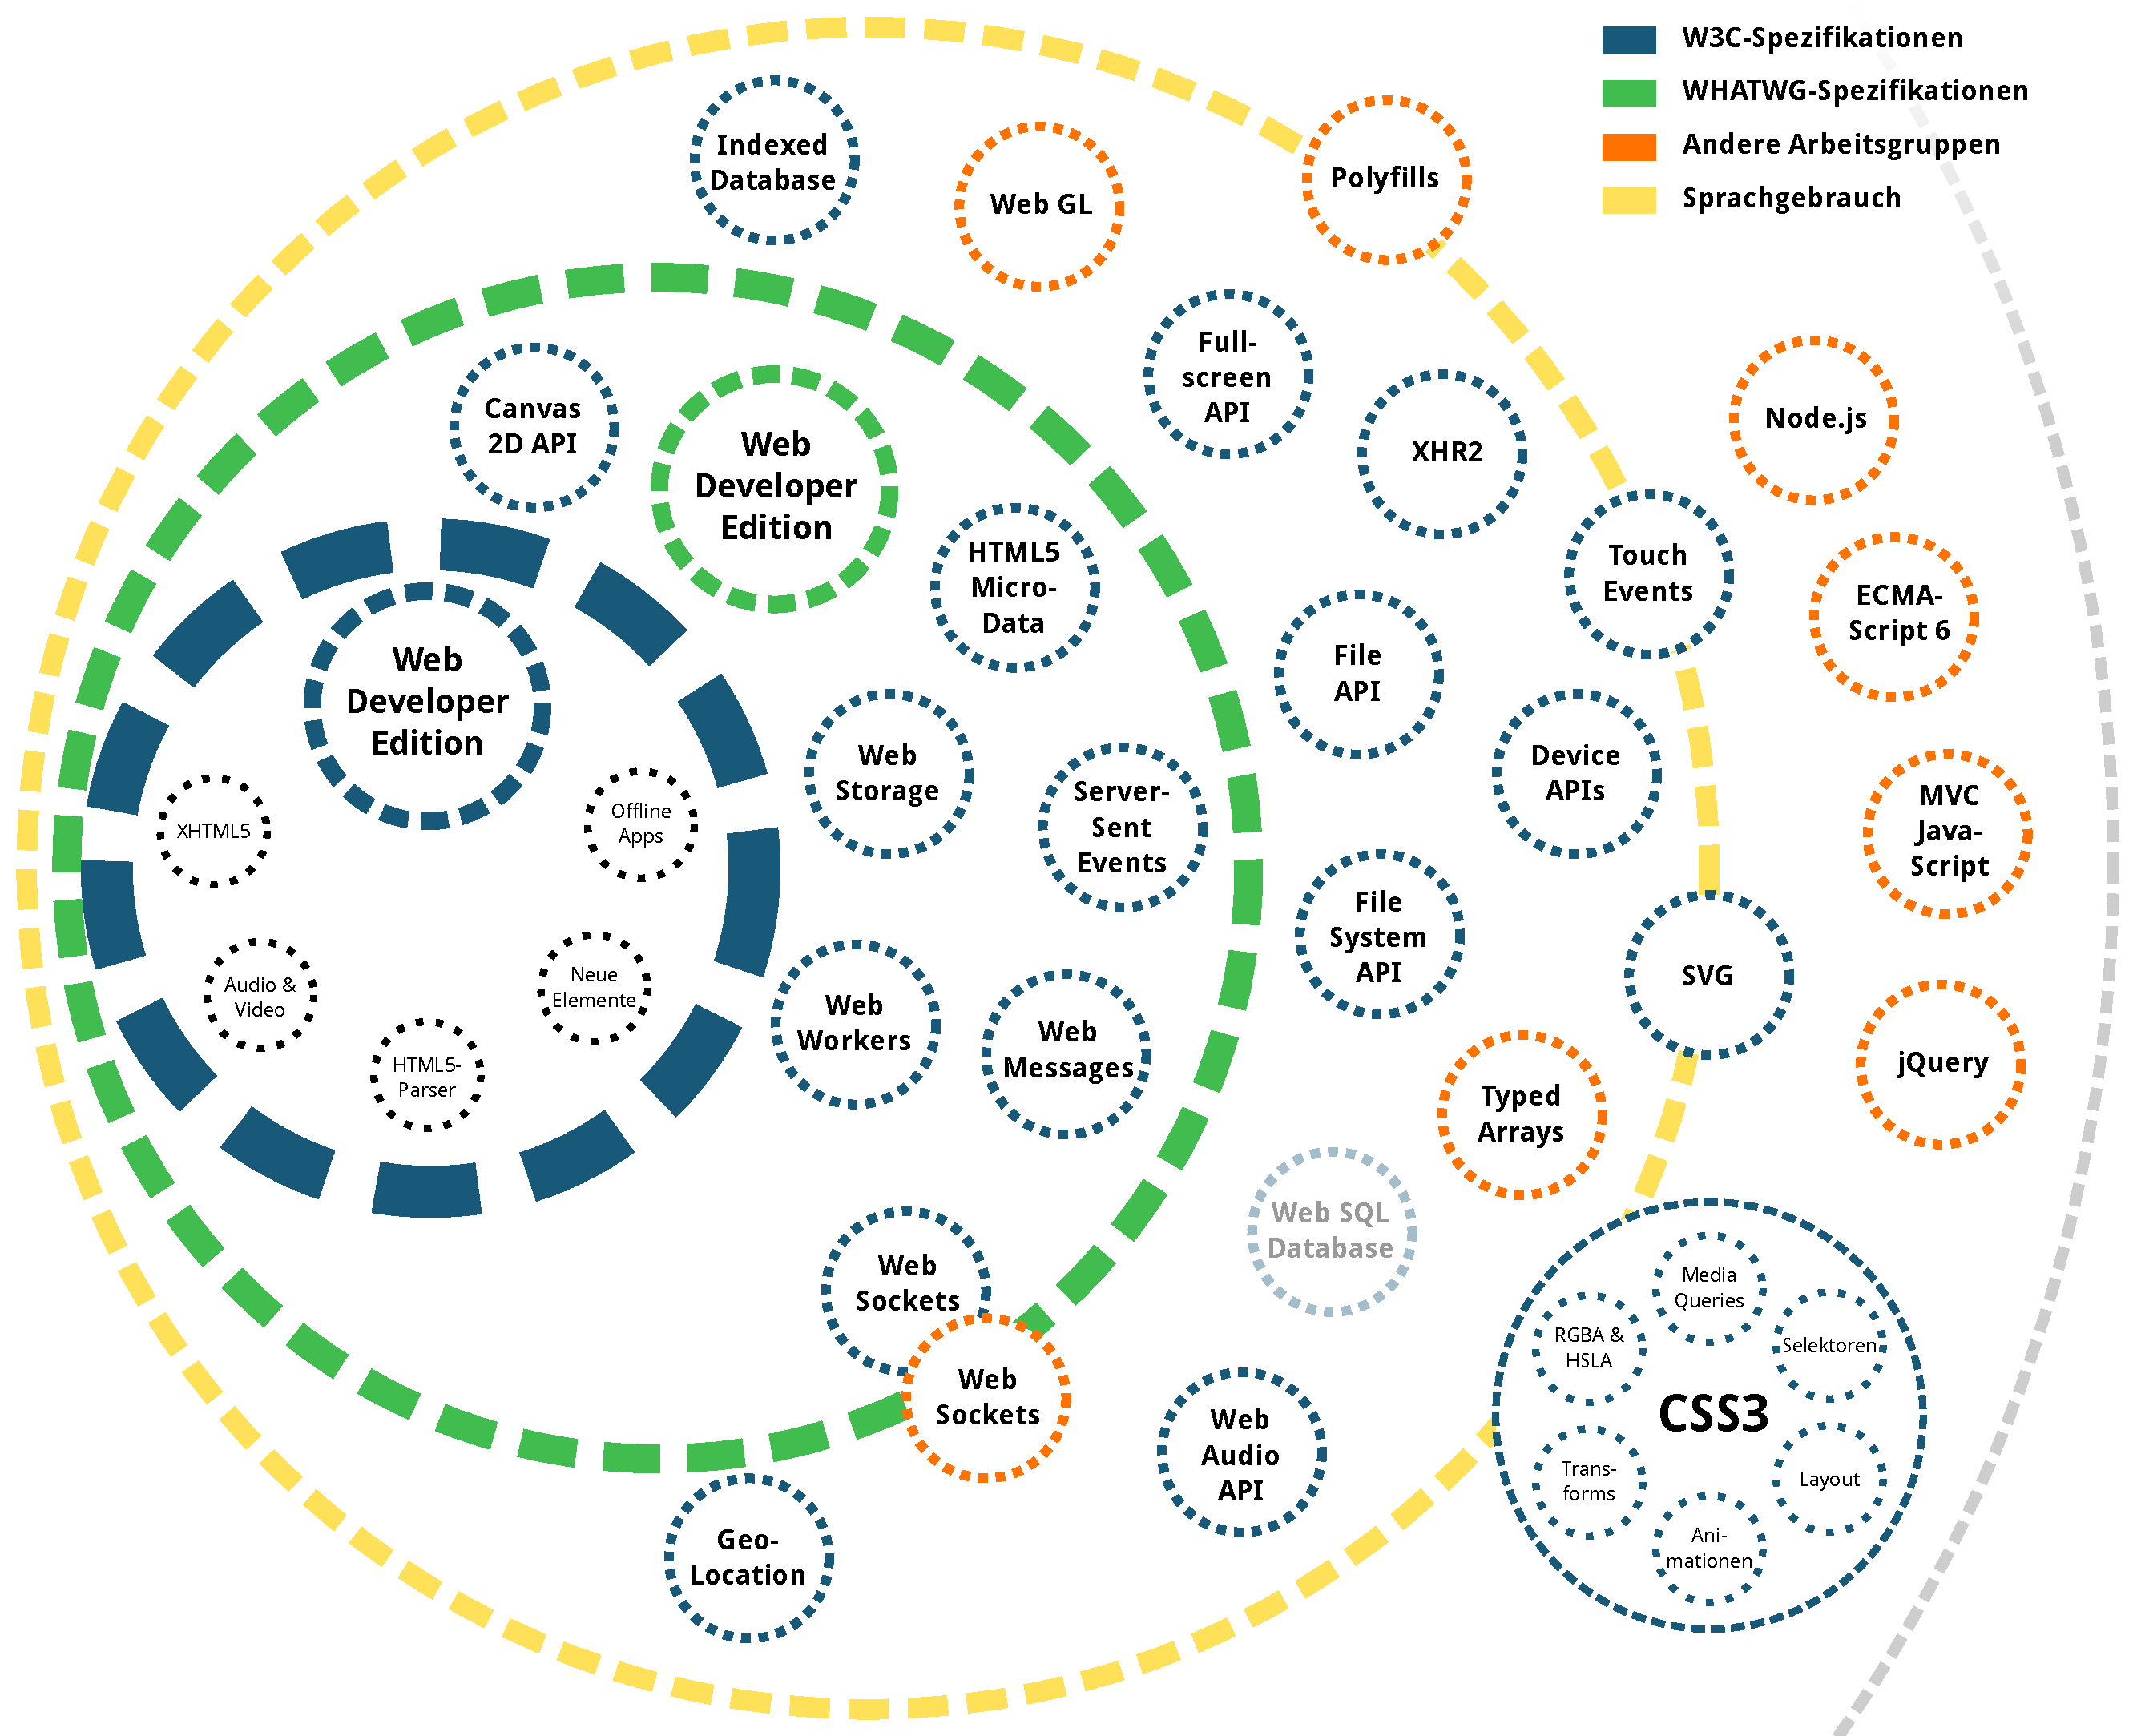
\includegraphics[width=\textwidth]{media/specGraph.pdf}
\caption{HTML5 Spezifikations-�bersicht (CC-BY-3.0 Peter Kr�ner) \cite{specGraph}}
\label{specgraphfig}
\end{figure}



Eine der Design-Entscheidungen bei der Entwicklung von HTML5 ist, den bestehenden Standard HTML 4.01 nicht zu ersetzen, sondern weiterzuentwickeln. Dadurch entsprechen die meisten Webseiten im HTML-4.01-Standard nach Anpassung der Dokumententypdeklaration direkt dem HTML5-Standard. \ref{diveInto}

Die Spezifikation hat den Status ``Last Call''\footnote{Stand: 22. August 2012}. Damit fordert das W3C auf letzte �nderungsvorschl�ge einzureichen, bevor der Standard im Jahr 2014 den Status ``Recommendation'' erhalten soll und damit final ist. Da jedoch die Implementierung in den einzelnen Browsern weit fortgeschritten ist und kaum noch �nderungen am Standard erwartet werden, kann er bereits jetzt eingesetzt werden. \cite{w3cpr}


\subsubsection{DOM und JavaScript APIs}

Nach dem parsen bildet der Browser intern die hierarchische Struktur eines HTML-Dokuments in Form eines Baumes ab. Diese Abbildung wird als \emph{Document Object Model (DOM)} bezeichnet. Der Zugriff auf den DOM-Baum ist mittels einer Schnittstelle (\emph{Application Programmable Interface (API)}) f�r JavaScript-Anwendungen m�glich. Elemente, Attribute und Texte sind als Knoten-Objekte angelegt und k�nnen ausgelesen oder manipuliert werden. \ref{mozdom}

Mit der zunehmenden Nutzung von Web-Applikationen sind auch die Anforderungen an die Browser gestiegen. Zur besseren Interaktion des Nutzers mit dem Browser wurden im Umfeld des HTML5-Standards viele weitere JavaScript-APIs definiert und vom W3C standardisiert (vgl. Abbildung \ref{specgraphfig}). \ref{keith} \ref{diveInto}



\subsubsection{Das canvas-Element}
\label{canvasapi}
Das \emph{canvas}-Element, wie in HTML5 definiert, ist ein rechteckiges Blockelement, das ohne weitere Anweisungen komplett unsichtbar ist: Es hat keinen sichtbaren Rahmen und der Inhalt des Elements ist transparent. In einem Dokument k�nnen sich beliebig viele canvas-Elemente befinden, die komplett unabh�ngig von einander sind. Jedes canvas ist im DOM-Baum verankert und kann mit einer ID versehen werden. Innerhalb des canvas-Elements kann alternativer Inhalt angegeben werden, der angezeigt wird wenn der Browser die Darstellung von canvas-Elementen nicht unterst�tzt. Eine beispielhafte Nutzung des Elements kann wie folgt aussehen: \ref{keith} \ref{diveInto}
\begin{verbatim}
    <canvas id="c" width="300" height="200">Fallback</canvas>
\end{verbatim}
Das Element definiert ein aufl�sungsabh�ngiges Bitmap, das in Echtzeit mit Grafikinhalten gef�llt werden kann. Laut Spezifikation definiert canvas einen JavaScript-Funktionsaufruf \verb+canvas.getContext(contextId [, ... ])+ bei dem ein Schl�sselwort in Form eines Strings als \verb+contextId+ �bergeben wird. \cite{W3Ccanvas} Die \emph{WHATWG} spezifiziert zwei m�gliche Kontexte: \verb+2d+ und \verb+webgl+. \cite{WHATWGcanvasContext} Der Funktionsaufruf liefert ein Objekt zur�ck das die jeweilige API bereitstellt oder \verb+null+ falls ein entsprechender Kontext nicht unterst�tzt wird.

Mittels der 2D-API k�nnen einfache Zeichenoperationen ausgef�hrt werden. Dazu geh�ren Linien, Pfade, Rechtecke, Ellipsen, aber auch Texte oder Bilder k�nnen eingef�gt werden. All diese Operationen werden direkt in der CPU berechnet und sind somit nicht hardwarebeschleunigt. Animationen k�nnen durch st�ndiges Neuzeichnen mittels JavaScript-Timer-Funktionen realisiert werden. \ref{WHATWGcanvas} \ref{diveInto}

\label{initwebgl}


% http://www.whatwg.org/specs/web-apps/current-work/multipage/the-canvas-element.html#drawing-text-to-the-canvas
% http://www.peterkroener.de/was-ist-html5-und-was-nicht-und-was-haette-der-kaiser-dazu-gesagt/
\chapter{Dreidimensionale Computergrafik im Browser}

\section{Historische Entwicklung der 3D-Technologie im Web}
\label{hist}

Erste Bem�hungen dreidimensionale Inhalte in den Webbrowser zu bringen begannen im Jahr 1994. Angelehnt an die Nutzung von HTML f�r die Darstellung von Webseiten sollte eine Auszeichnungssprache f�r die Darstellung dreidimensionaler Inhalte geschaffen werden. Anforderungen an die neue Sprache waren Plattformunabh�ngigkeit, Erweiterbarkeit und Nutzbarkeit auch bei geringer Internet-Bandbreite. Das zu diesem Zweck gegr�ndete \emph{Web3D}-Konsortium entwickelte die \emph{Virtual Reality Modeling Language (VRML)}. Am 26. Mai 1995 wurde die finale Spezifikation von \emph{VRML 1.0} ver�ffentlicht. Dort wird ein einfaches textbasiertes Format definiert, in dem Objekte geschachtelt abgelegt werden k�nnen. Diese Objekte k�nnen Kameras, Lichter, Materialien, aber auch dargestellte 3D-Objekte oder Transformationen sein. Zur Speicherung der Szenen wird die Dateiendung \verb+.wrl+ (f�r engl. \emph{world}) vorgegeben. \cite{vrml10} 1997 wurde \emph{VRML 2.0 (VRML97)} fertiggestellt und als ISO-Standard 14772-1:1997 definiert. Unter anderem wurde der VRML-1.0-Standard um Animationen und Nutzerinteraktionsm�glichkeiten erweitert. \cite{vrml97} \cite{vrml972}

F�r die Darstellung von VRML-Inhalten gibt es einige Browser-Plugins, jedoch integrierete nahezu kein Browser-Hersteller den Standard direkt in sein Produkt. In den folgenden Jahren entstanden viele weitere Dateiformate zur Speicherung von 3D-Szenen mit Augenmerk auf die Darstellung im Browser. Unter anderem trat das XML-basierte Format \emph{X3D} die Nachfolge von VRML an. Das Web3D-Konsortium schl�gt vor den X3D-Standard komplett in HTML5 zu integrieren, jedoch hat das W3C das bisher abgelehnt: \emph{``Embedding 3D imagery into XHTML documents is the domain of X3D, or technologies based on X3D that are namespace-aware.''} \cite{nox3d} �hnlich wie bei \emph{SVG} oder \emph{MathML} soll so eine native Darstellung ohne Plugin erm�glicht werden. \cite{x3domhtml}



\section{Deklarative und imperative 3D-Darstellung in Browsern}


Die Darstellung von zwei- und dreidimensionalen Grafiken im Browser kann grundlegend auf zwei verschiedene Arten erfolgen: Zum einen ist es m�glich den Szenengraph als Teil des HTML-Dokuments zu deklarieren. Somit sind die einzelnen Objekte der Grafik gleichberechtigt mit HTML-Elementen auf der Seite. Jedes Objekt der Grafik ist im DOM-Baum integriert und kann per CSS oder JavaScript selektiert und modifiziert werden. Zur Darstellung zweidimensionaler Grafiken ist das \emph{SVG}-Format im HTML5-Standard aufgenommen. Das �quivalent f�r dreidimensionale Grafiken, X3D, ist wie in Kapitel \ref{hist} beschreiben nicht Teil des Standards. \cite{x3dom} 

Zum anderen k�nnen Grafiken imperativ auf eine Zeichenfl�che gezeichnet werden. Als Zeichenfl�che wird das canvas-Element genutzt und ist dabei das einzige Objekt der Grafik, das im DOM-Baum verankert ist. Inhalte die auf die Zeichenfl�che gezeichnet wurden k�nnen nicht mehr ver�ndert werden. Die Zeichenfl�che kann lediglich komplett oder in Ausschnitten geleert und/oder �berzeichnet werden. HTML5 definiert die 2D-F�higkeiten des canvas-Elements und Verwendung von WebGL f�r 3D-Inhalte. \cite{2dcontext}

\begin{table}[h]

\centering
\begin{tabular}{l||c|c}
     & \textbf{2D} & \textbf{3D} \\
\hline
\hline
    \textbf{Deklarativ} & SVG & X3D\footnotemark \\
\hline
    \textbf{Imperativ} & canvas & WebGL
\end{tabular}

\label{tbl:tablelabel}
\caption{Deklarative und imperative Grafikdarstellung im Web \cite{x3dom}}
\end{table}
\footnotetext{nicht vom W3C standardisiert}

%http://www.w3.org/TR/2dcontext/



\chapter{WebGL}


Die \emph{Khronos Group} ist ein Konsortium aus �ber 100 Firmen, die es sich seit Januar 2000 zum Ziel gesetzt hat, offene Standards f�r Mediendarstellung auf Computern, mobilen Ger�ten und in integrierten Systemen zu definieren. Als gemeinn�tzige Organisation arbeitet die Gruppe nicht gewinnorientiert und finanziert sich lediglich aus den j�hrlichen Beitr�gen ihrer Mitglieder. In verschiedenen Arbeitsgruppen sollen Industrie-Standards entwickelt und linzenzfrei zur Verf�gung gestellt werden. Dazu gibt es das \emph{Khronos IP Framework}--eine Vereinbarung zwischen den Khronos-Mitgliedern, keine Patentstreitigkeiten bez�glich der Khronos-Standards gerichtlich auszutragen. \cite{KhronosAbout}

Der �lteste Standard der Khronos-Gruppe ist \emph{OpenGL (Open Graphics Library)}, der 1992 von \emph{Silicon Graphics Inc. (SGI)} entwickelt wurde. OpenGL spezifiziert eine hardwareunabh�ngige Software-Schnittstelle (API) zum Grafikprozessor mit mehreren hundert Befehlen, einer kleinen Menge geometrischer Primitive und einer eigenen Shader-Programmiersprache \emph{OpenGL Shading Language (GLSL)}. Die meisten gro�en Betriebssysteme, darunter Windows, Mac OS und Linux, unterst�tzen OpenGL. \cite{Shreiner} \cite{SGI} \cite{KhronosAbout2}

Als propriet�re Alternative zu OpenGL bietet Microsoft \emph{Direct3D} f�r die Windows- und XBox-Plattform an. Zudem gibt es eine angepassten Version f�r Microsofts mobiles Betriebssystem \emph{Windows Phone Series}.

Ausgehend vom OpenGL-Standard entwickelte die Khronos Group einen weiteren Standard: \emph{OpenGL for Embedded Systems (OpenGL ES)} ist eine Teilmenge von OpenGL, die speziell f�r den Einsatz auf mobilen Ger�ten wie etwa Smartphones oder Spielekonsolen entwickelt wurde und eine hohe Verbreitung unter anderem in Googles Android \cite{devGoogle} oder Apples iOS \cite{devApple} findet. Applikationen die gegen OpenGL ES geschrieben wurden laufen auch unter der entsprechenden Version von OpenGL. Andersherum ist das nicht der Fall.


WebGL bringt nun die M�glichkeit OpenGL-ES-2.0-Inhalte im Browser darzustellen und dabei die Hardware-Beschleunigung der Grafikkarte zu nutzen. Bisher konnten Webinhalte lediglich den Hauptprozessor (CPU) f�r ihre Berechnungen nutzen. Grafikkarten sind hochgradig f�r die typischen Berechnungen von 3D-Darstellungen optimiert und k�nnen die Prozessorleistung bei weitem �bertreffen. Mittels der WebGL-Technologie k�nnen Applikationen die zum Beispiel f�r mobile Ger�te konzipiert wurden ohne gr��ere Anpassungen im Browser ausgef�hrt werden. Die Anwendungsgebiete sind vielf�ltig: Von Visualisierungen, Simulationen, Spielen, bis zu Kunst ist alles denkbar. \cite{operawebgl} \cite{webgl}


\section{Technik und Funktionsumfang}
\label{tecandfunc}
Die WebGL-Programmierung erfolgt in JavaScript und die Programmierung der Shader in GLSL, deren Syntax �hnlich zu JavaScript ist. Shader sind das grundlegende Konzept von WebGL und OpenGL. Dabei handelt es sich um Unterprogramme, die in der Grafikkarte ausgef�hrt werden und �ber die Darstellung der 3D-Szene entscheiden. In WebGL gibt es mit Vertex- und Fragment-Shader zwei unterschiedliche Arten, deren Funktionsweise in Kapitel \ref{pipeline} erl�utert wird. Die Shader k�nnen frei programmiert werden, aber viele Grafikbibliotheken bringen bereits vordefinierte Shader mit (vgl. Kapitel \ref{webglbib}).

Das canvas-Element wird als Zeichenfl�che f�r die WebGL-Inhalte verwendet. Wie jedes andere HTML-Element kann das canvas-Element �ber oder unter anderen Elementen des Dokuments dargestellt werden. So ist auch die �berlagerung von HTML- und WebGL-Inhalten m�glich.

Mittels des in Kapitel \ref{initwebgl} beschriebenen Funktionsaufrufs kann die Initialisierung eines WebGL-Kontexts wie Listing \ref{webglinitcode} aussehen. \cite{html5rocks} Zun�chst wird der Funktionsaufruf der Initialisierung auf den \verb+onload+-Event-Listener gelegt (Zeile \verb+11+) und somit die Funktion \verb+init()+ beim Laden der Seite aufgerufen. Mittels der Element-ID wird das canvas-Element selektiert (Zeile \verb+3+) und dessen WebGL-Kontext aufgerufen (Zeile \verb+4+). Ist der Kontext nicht vorhanden, wird WebGL nicht unterst�tzt (Zeilen \verb+5+-\verb+7+), andernfalls steht dann der WebGL-Kontext �ber die Variable \verb+gl+ zur Verf�gung.

\begin{lstlisting}[caption=Initialisierung eines WebGL-Kontexts,label=webglinitcode]
<script type="text/javascript">
    function init() {
        canvas = document.getElementById("c");
        gl = canvas.getContext("webgl");
        if (!gl) {
            return; /*WebGL wird nicht unterst�tzt*/
        }
        ...
    }

    window.onload = init;
</script>
<canvas id="c"></canvas>
\end{lstlisting} 

Zus�tzlich k�nnen Vertex- und Fragment-Shader mit folgendem Mark-Up ausgezeichnet werden und dann in GLSL programmiert werden:

\begin{lstlisting}[caption=Deklaration der WebGL-Shader]
<script id="vshader" type="x-shader/x-vertex">
    ... /* Vertex-Shader */
</script>
<script id="fshader" type="x-shader/x-fragment">
    ... /* Fragment-Shader */
</script>
\end{lstlisting} 

WebGL verwendet ein eigenes kartesisches Koordinatensystem das unabh�ngig von der Gr��e und Aufl�sung des canvas-Elements ist. Der Wertebereich der x-, y- und z-Achse liegt im Intervall $[-1;1]$. Die x-Achse beginnt auf der linken Seite mit $-1$, die y-Achse hat den Wert $-1$ an der unteren Bildkante. Die z-Ache zur Tiefenbestimmung hat f�r die n�chsten Objekte den Wert $-1$ und f�r die entferntesten den Wert $1$. F�r die Darstellung auf dem Bildschrim werden die WebGL-Koordinaten dann auf die canvas-Koordinaten umgerechnet.


\subsection{Die WebGL-Rendering-Pipeline}
\label{pipeline}
Folgende Schritte werden bei der Berechnung eines Bilds bei der OpenGL-ES-/WebGL-Technologie durchlaufen. Der Ablauf ist vereinfacht dargestellt und weitaus identisch mit der Arbeitsweise anderer Grafik-Bibliotheken. \cite{beginnersGuide} \cite{operawebgl} \cite{Shreiner}

\begin{enumerate}
    \item Wie f�r 3D-Renderingprozesse �blich, verwendet WebGL polygonale Modellierung. Das bedeutet, dass Objekte aus Polygonen zusammengesetzt werden. �blicherweise und auch in WebGL werden daf�r Dreiecke verwendet. In JavaScript-Code wird nun eine Menge von Punkten (Vertices) definiert und in einem Array gespeichert. Zu jedem Vertex k�nnen neben der Position im dreidimensionalen Raum auch die Farbe, Transparenz und Texturkoordinaten gespeichert werden. Ein zweites Array ordnet die Indizes des Vertex-Arrays zu Dreiergruppen zusammen und gibt die Reihenfolge an, in der die Punkte zu Dreiecken zusammengesetzt werden.
    
    \item Das Vertex- und Index-Array werden dann an die Grafikkarte �bergeben. F�r jedes Vertex wird ein Unterprogramm, der so genannte \textbf{Vertex-Shader}, aufgerufen, der Operationen auf jedem einzelnen Vertex ausf�hren kann. Hier k�nnen Manipulationen an den Formen des Objekts vorgenommen werden. Au�erdem wird mit Hilfe einer Matrixmultiplikation die Projektion des dreidimensionalen Punkts auf die zweidimensionale Fl�che zur Anzeige auf dem Bildschirm berechnet. 
        
    \item Anschlie�end wird in der Grafikkarte das Bild \textbf{rasterisiert}. Dabei wird die zweidimensionale Projektion mit einem Pixelraster der Gr��e des canvas-Elements �berlagert und jeder Punkt einem Pixel zugeordnet. Hier k�nnen auch Kantengl�ttungs-Mechanismen (Antialiasing) angewendet werden. Die Farben zwischen zwei Vertices k�nnen mit Hilfe der zugeh�rigen Farbwerte interpoliert werden.
    
    \item F�r jedes berechnete Pixel wird nun ein weiteres Unterprogramm aufgerufen: Der \textbf{Fragment-Shader} kann die Farbewerte des jeweiligen Pixels ver�ndern und sorgt somit f�r die Darstellung von Texturen, Oberfl�chenmaterialien, Lichtern und Schatten.
    
    \item Das fertige Pixelbild wird im \textbf{Frame-Buffer} der Grafikkarte abgelegt und kann von dort aus dann im canvas-Element der Webseite dargestellt werden.
\end{enumerate}


\section{Verbreitung und Implementierung in den verschiedenen Browsern}

Mitglieder der Khronos Group sind mit Google (Chrome), Apple (Safari), Mozilla (Firefox) und Opera unter anderem einige namenhafte Browser-Hersteller, die gemeinsam an der Entwicklung von WebGL arbeiten. Deshalb geschieht die Adaption neuer Funktionen in den genannten Browsern meist schnell und fl�chendeckend.

\subsection{Vergleich der WebGL-F�higkeiten ausgew�hlter Browser}

F�r den Vergleich wurden die f�nf Browser mit den gr��ten Marktanteilen herangezogen. Gemeinsam decken diese f�nf Browser 98,41\%\footnote{Stand: Juli 2012} des Desktop-Marktes ab. \cite{StatTop5Browser} Mobile Browser sind in diesem Vergleich ausgenommen und werden gesondert in Kapitel \ref{mobilewebGL} behandelt. 

Der \emph{WHATWG}-Standard \cite{WHATWGcanvas} gibt f�r den Aufruf der Schnittstelle des WebGL-Kontexts das Schl�sselwort \verb+webgl+ vor, jedoch implementieren die verglichenen Browser alle ausschlie�lich das Schl�sselwort \verb+experimental-webgl+ und liefern f�r den Kontext \verb+webgl+ den Wert \verb+null+ zur�ck.\footnote{Stand: August 2012 (Chrome 21, Firefox 14, Safari 6.0, Opera 12.00)} Solange die Spezifikation nicht final ist und der Standard nicht vollst�ndig implementiert wurde wird dieses Vorgehen vom \emph{W3C} und der \emph{WHATWG} empfohlen. \cite{W3Ccanvas} \cite{WHATWGcanvas}


\subsubsection{Microsoft Internet Explorer}

Microsoft stuft die Implementierung von WebGL als zu gef�hrlich ein und verzichtet deshalb auf eine Integration in den \emph{Internet Explorer}. Problematisch sieht Microsoft dabei die direkte Bereitstellung der Grafikkarte f�r beliebige Webseiten-Betreiber. Sicherheitsl�cken in Grafikkarten-Treibern die bisher nur lokal ausgenutzt werden konnten, stehen somit f�r das Internet offen (vgl. Kapitel \ref{webglsec}). \cite{MSWebGL} Als alternative Technologie schl�gt Microsoft die Eigenentwicklung \emph{Silverlight} vor, die seit der Version 5 ebenfalls hardwarebeschleunigte 3D-Darstellung unterst�tzt. \cite{Silverlight}

Dennoch l�sst sich mittels Plugin eines Fremdanbieters die Unterst�tzung f�r WebGL ab Internet Explorer Version 8 nachr�sten. \cite{IEWebGL}




\subsection{Marktanteile der Webbrowser}

\begin{table}[h]

\centering
\begin{tabular}{l|rrcr}
    \textbf{Browser} &   \vbox{\hbox{\strut \textbf{Marktanteil}}\hbox{\strut \verb+     +\textbf{gesamt}}} & \vbox{\hbox{\strut \textbf{WebGL ab}}\hbox{\strut \verb+  +\textbf{Version}\footnotemark}} & \textbf{Release} & \vbox{\hbox{\strut \verb+ +\textbf{Marktanteil}}\hbox{\strut \textbf{WebGL-f�hig}}}\\
\hline
\hline
    Google Chrome & 33,29\% & 9.0 & 03.02.2011 \cite{releaseChrome} & 32,89\% \\
\hline
    Internet Explorer & 32,17\% &\multicolumn{2}{r}{\textit{keine WebGL Unterst�tzung}} & 0,00\% \\
\hline
    Mozilla Firefox & 24,14\% & 4.0 & 22.03.2011 \cite{releaseFirefox} & 22,13\%\\
\hline
    Apple Safari & 7,06\% & 5.1 & 20.07.2011 \cite{releaseSafari} & 3,41\%\\
\hline
    Opera & 1,75\% & 12.00 & 14.06.2012 \cite{releaseOpera} & 0,78\%\\
\hline
\hline
    \textbf{Summe} & \textbf{98,41\%} & & & \textbf{59,21\%} \\
\end{tabular}

\caption{Marktanteile der f�hrenden Webbrowser\cite{StatTop5Browser} \cite{statVersion}}
\label{marketshare}
\end{table}

\footnotetext{F�r den Vergleich wurden nur finale Versionen der jeweiligen Browser herangezogen. Alpha-, Beta- und Preview-Versionen sind ausgenommen und waren teilweise schon wesentlich fr�her verf�gbar.}


Basierend auf den Zahlen von StatCounter.com f�r Juni bis Juli 2012 haben WebGL-f�hige Browserversionen einen Marktanteil von 59,21\% (vgl. Tabelle \ref{marketshare}). Jedoch muss der Anteil der Browser, die WebGL-Inhalte korrekt darstellen geringer angegeben werden, da durch Inkompatibilit�ten mit speziellen Grafikkarten einige Browserversionen WebGL deaktivieren. Hinzu kommt, dass Safari mit deaktiviertem WebGL ausgeliefert wird, welches erst vom Benutzer manuell aktiviert werden muss. Daher lassen sich ohne eigener Erhebung dieser Daten keine verl�sslichen Aussagen �ber die genaue Verbreitung von Browsern mit aktivierter WebGL-F�higkeit treffen.




\subsection{Mobile Verf�gbarkeit von WebGL} \label{mobilewebGL}

Es wurde die Verf�gbarkeit des WebGL-Standards auf den beiden f�hrenden mobilen Betriebssystemen verglichen. \cite{mobileos} Dabei wird die grundlegende Verf�gbarkeit der OpenGL-Technologie sowie die Implementierung der WebGL-Technologie im mitgelieferten Browser betrachtet. 

\subsubsection{Apple iOS und Mobile Safari}

Apple implementiert in iOS\footnote{Stand: iOS 5.1.1} OpenGL ES 1.1 und 2.0 f�r die Darstellung von 2D- und 3D-Inhalten. Applikationsentwickler k�nnen die Standards f�r die Darstellung ihrer Inhalte nutzen. \cite{iosopengl} Jedoch ist die Nutzung von OpenGL in Form von WebGL im systemeigenen Browser \emph{Mobile Safari} nicht m�glich. F�r in Applikationen eingebettete Web-Darstellungen l�sst sich WebGL aktivieren, jedoch widerspricht die Nutzung Apples Richtlinien f�r Entwickler. Lediglich innerhalb Apples webbasiertem Werbenetzwerk \emph{iAd} ist die Nutzung von WebGL m�glich. Au�erdem kann die Darstellung von \emph{CSS3-Animationen} im Browser auf Hardwarebeschleunigung zur�ckgreifen. \cite{devApple}

\subsubsection{Android}

F�r die Entwicklung von Applikationen unterst�tzt die Android-Plattform ebenso den OpenGL ES 1.1 und ab Android 2.2 (API Level 8) auch den OpenGL ES 2.0 Standard. \cite{devGoogle} WebGL ist im Android Browser nicht verf�gbar. Sony entwickelte eine Modifikation f�r den Android Browser die WebGL implementiert. \cite{sonywebgl} Diese wird bisher nur auf dem \emph{Sony Xperia} Smartphone eingesetzt.

\section{Sicherheit in WebGL}
\label{webglsec}

Im Mai 2011 beschrieb \emph{Context Information Security} mehrere m�gliche Angriffsszenarien mit Hilfe von manipulierten WebGL-Inhalten. \cite{contextwebgl} Generell stellt WebGL ein hohes Bedrohungspotential dar, da es den direkten Zugriff von Webseiten auf die Hardware des Rechners zul�sst. Nat�rlich versuchen Browserhersteller, die Khronos Group und die Grafikkartenhersteller diese Angriffe zu verhindern, trotzdem sind diverse Szenarien denkbar, in denen WebGL dazu genutzt werden kann den Rechner anzugreifen.

\subsection{Denial-of-Service-Attacken}

Mittels sehr komplexer 3D-Geometrien oder extrem aufw�ndiger Shaderprogramme wird die Grafikkarte so lange beansprucht, dass weder andere Programme noch das Betriebssystem die Grafikkarte nutzen k�nnen und der Rechner so unter Umst�nden abst�rzt oder unbenutzbar wird. \cite{contextwebgl2} Gegen diese Art von Angriff wurden bisher kaum Ma�nahmen ergriffen. Seit Windows Vista implementiert Microsoft einen Sicherheitsmechaniasmus, der die Grafikkarte zur�cksetzt, wenn diese f�r �ber zwei Sekunden nicht mehr reagiert. \cite{windows} Dieses Vorgehen schl�gt auch die Khronos Group f�r OpenGL-kompatible Grafikkarten in der Erweiterung \emph{GL\_ARB\_robustness} vor, jedoch haben noch nicht alle Grafikkartenhersteller diese Erweiterung implementiert. Somit sind aktuell viele System f�r diese Art von Angriff gef�hrdet. \cite{KhrSec}

% http://msdn.microsoft.com/en-us/windows/hardware/gg487368.aspx
% http://www.khronos.org/news/permalink/webgl-security

\subsection{Zugriff auf den Frame-Buffer}

Die WebGL-Technologie erm�glicht Webseiten den Zugriff auf den Inhalt des Frame-Buffers der Grafikkarte. Der Frame-Buffer ist ein gemeinsam genutzter Speicherbereich in dem alle auf dem Bildschirm dargestellten Inhalte liegen. Deshalb ist laut Spezifikation der Zugriff auf den Teil des Frame-Buffers beschr�nkt, der den Inhalt des canvas-Elements speichert. Jedoch kam es durch fehlerhafte Implementierungen des WebGL-Standards und Bugs in Grafikkarten-Treibern dazu, dass auch andere Inhalte des Frame-Buffers in das canvas-Element gezeichnet werden konnten. So konnten Informationen ausgelesen werden, die der Nutzer beispielsweise in anderen Applikationen oder auf seinem Desktop dargestellt hat. Seitens Khronos Group un der Grafikkartenhersteller wurden diese Fehler behoben. Es ist jedoch nicht ausgeschlossen, dass durch neue Sicherheitsl�cken dieser Angriff wieder erm�glicht wird. \cite{contextwebgl2}

\subsection{Cross-Domain Texturen}

Das Nachladen externer Modelle oder Texturen kann den Zugriff auf fremde Ressourcen erfordern. Ein Sicherheitskonzept, das mit \emph{Netscape Navigator 2.0} f�r clientseitige Skriptsprachen, wie beispielsweise JavaScript, eingef�hrt wurde ist die \emph{Same-Origin-Policy (SOP)}. Diese verbietet clientseitige lesende Zugriffe, zum Beispiel per \emph{XMLHttpRequest}, auf fremde Ressourcen. Sie verlangt, dass Zugriffe innerhalb einer Webseite nur auf Ressourcen der selben Domain, �ber den selben Port mittels des selben Protokolls erfolgen d�rfen. Das betrifft nicht das Einbinden fremder Inhalte, wie das Einbetten eines Bildes, sondern den lesenden Zugriff eines Skripts auf solche Inhalte. Durch einen clientseitigen lesenden Zugriff k�nnten Informationen von fremden Seiten ausgelesen werden. H�tte ein Nutzer beispielsweise eine Banking-Seite ge�ffnet, k�nnte eine andere Seite deren Inhalte einlesen und zu einem fremden Server �bertragen. Daher wird der clientseitige lesende Zugriff im Normalfall auf die jeweilige Domain beschr�nkt. \cite{MDNsop}

Um dennoch entfernte Ressoucen nutzen zu k�nnen wurde \emph{Cross-Origin-Resource-Sharing (CORS)} entwickelt. Dabei gibt der ausliefernde Server in seinem HTTP-Header an, welche fremden Seiten seine Ressourcen lesen d�rfen. Dabei ist auch die Verwendung einer Wildcard m�glich um den lesenden Zugriff f�r alle fremden Seiten zuerm�glichen. \cite{cors} \cite{corsbug}




\section{WebGL-Bibliotheken}
\label{webglbib}
Um den Umgang mit WebGL zu vereinfachen gibt es einige Bibliotheken. Diese stellen beispielsweise geometrische Grundformen wie W�rfel, Kugeln, Zylinder, etc. zur Verf�gung. Au�erdem lassen sich somit WebGL-Aufrufe mittels JavaScript ausf�hren, ohne eigenen Shader-Code in \emph{GLSL} nutzen zu m�ssen. Komplexe mathematische Berechnungen die f�r die Realisierung verschiedener Kameras m�ssen nicht in einem eigenen Vertex-Shader realisiert werden, sondern k�nnen als fertige Programme geladen werden. Ebenso ist f�r die Realisierung von Oberfl�chenmaterialen und Beleuchtungsmodellen keine Programmierung eines eigenen Fragment-Shaders n�tig, da g�ngige Materialien und Beleuchtungsmodelle bereits als vordefinierte Shader vorhanden sind. F�r die meisten Anwendungsf�lle reicht die Nutzung der durch Kamera-, Material- und Beleuchtungsobjekten vordefinierten Shader aus und es muss kein Shadercode geschrieben werden. Die Programmierung kann dann ausschlie�lich in JavaScript erfolgen. Zus�tzlich k�nnen unterschiedliche Implementierungen verschiedener Browser angefangen und f�r den Programmierer unsichtbar gemacht werden.

\subsection{die THREE.js-Bibliothek}

Entwickelt von \emph{Ricardo Cabello Miguel} ist \emph{THREE.js} eine der am weitesten verbreiteten Bibliotheken f�r WebGL. Seit 2010 wird THREE.js entwickelt und befindet sich aktuell in der Version r50\footnote{Stand: 19. August 2012}. Einige elementare Bestandteile der Bibliothek sollen im Folgenden vorgestellt werden. \cite{threejsdocs}

\begin{itemize}
\item \textbf{Renderer:} Neben der Ausgabe in den \verb+webgl+-Kontext, ist in einem begrenzen Ma�e auch die Ausgabe in eine \emph{SVG}-Datei, oder in den \verb+2d+-Kontext des canvas-Elements m�glich. Jedoch ist nur die WebGL-Ausgabe hardwarebeschleunigt. F�r nicht WebGL-f�hige Browser kann in einigen Anwendungsf�llen eine der alternativen Ausgaben genutzt werden.

\item \textbf{Kameras:} THREE.js hat zwei verschiedene Kamera-Objekte zur Verf�gung. Eine orthographische Kamera die eine parallele Projektion auf die Sichtebene vornimmt, sowie eine persketivische Kamera, die dem Verhalten des menschlichen Auge entspricht. Hierbei wird das Sichtfeld mit einem Winkel angegeben.

\item \textbf{Geometische Primitive:} Einige geometische Primitive sind in der Bibliothek bereits angelegt und k�nnen verwendet werden. Darunter befinden sich: W�rfel, Zylinder, Ebene, Kugel und Torus.

\item \textbf{Lichter:} In THREE.js sind verschiedene Lichter definiert, die sich unterschiedlich auf die Szene auswirken. Das \verb+AmbientLight+ hellt die gesamte Szene auf, hat keine Richtung und wirft keine Schatten. Das \verb+DirectionalLight+ ist gerichtet, hat aber keinen Ursprung. Das Licht verl�uft parallel und wirft Schatten. \verb+SpotLight+ und \verb+PointLight+ haben eine punktf�rmige Position. Beide strahlen das Licht kugelf�rmig ab, wobei es linear abgeschw�cht wird. Nur SpotLights k�nnen Schatten werfen. 

\item \textbf{Oberfl�chenmaterialien:} Die unterschiedlichen Oberfl�chenmaterialien wirken sich auf das Verhalten von Licht auf den Objekten aus. Das \verb+BasicMaterial+ ignoriert einfallendes Licht und stellt das Objekt gleichm��ig in der angegebenen Farbe dar. F�r die realistische Darstellung bieten sich \verb+PhongMaterial+ und \verb+LambertMaterial+ an, die einfallendes Licht nach den jeweiligen Beleuchtungsmodellen verarbeiten und so die Farbdarstellung berechnen. Zus�tzlich ist es m�glich Grafiktexturen auf Objekten abzubilden.


\end{itemize}











\chapter{Fu�g�ngersimulation und Visualisierung}


Bei der Planung von Gro�veranstaltungen oder der Konzeption neuer Geb�ude werden Fu�g�ngersimulationen eingesetzt um Evakuierungsszenarien zu simulieren und ggf. Katastrophen vorzubeugen. Analysen und Simulationen, warum beispielsweise auf Autobahnen ein Stau entsteht, sind mittlerweile problemlos machbar. Die Vorhersage, welchen Weg ein Fu�g�nger einschlagen wird ist dagegen ein gr��eres Problem. W�hrend sich Autos auf festen Fahrbahnen bewegen und sich wesentlich strikter an Verkehrsregeln halten, haben Fu�g�nger mehr Freiheitsgrade in ihrer Bewegung. Spontan k�nnen sich Fu�g�nger dazu entschlie�en die Richtung zu �ndern, versuchen Gedr�nge aus dem Weg zu gehen und verlieren sogar manchmal ihr Ziel aus den Augen.

Um das Verhalten der Fu�g�nger zu simulieren werden verschiedene Verfahren angewandt. Ein popul�res Modell ist aus der Str�mungslehre entliehen. Es betrachtet einen einzelnen Fu�g�nger wie ein Molek�l in der Luft, das sich durch eine Str�mung bewegt. Wie Gase k�nnen Fu�g�nger nicht beliebig zusammengepresst werden. Dieses Modell funktioniert aber bei weniger dicht gedr�ngten Szenarien nicht mehr. Ein anderes Modell sind zellul�re Automaten. Dabei wird die zur Verf�gung stehende Fl�che schachbrettartig eingeteilt, wobei jedes Feld entweder von einer Person belegt oder frei sein kann. Anhand des aktuellen Zustands wird dann die Belegung im folgenden Schritt berechnet. \cite{spon1}

Au�erdem spielen bei den Wegen von Fu�g�ngern noch andere Faktoren mit. So gibt es beispielsweise einen kulturell gepr�gten Mindestabstand zu anderen Personen, der in Asien meist h�her ist als in Europa, in S�damerika dagegen geringer. Soziale Konventionen und unterbewusste Entscheidungen haben ebenso einen Einfluss auf die Wegewahl. Fu�g�nger passen ihre Geschwindigkeit der Masse an um einen Aufprall zu vermeiden, in einem Gedr�nge k�nnen sich Bahnen bilden, die sich in die selbe Richtung bewegen und in Paniksituationen k�nnen sich Menschen komplett irrational verhalten. \cite{spon1}

Ein viel zitierter Extremfall ist das Ungl�ck auf der ``Love Parade'' am 24.07.2010 bei dem 21 Personen im Gedr�nge der panischen Menschenmassen zu Tode kamen. Dieses Ereignis hat sicherlich das Bewusstsein um die Notwendigkeit akurater Simulationen gest�rkt, um so Engstellen und potentielle Gefahrenpunkte schon im Vorfeld zu erkennen und durch Sicherheitskr�fte oder bauliche Ma�nahmen zu entsch�rfen. \cite{spon2}

In dieser Arbeit wird die Erstellung einer dreidimensionalen webbasierten Visualisierung von Fu�g�ngersimulationsdaten beschrieben. Die Ergebnisse der Simulationen sind als Webapplikation �berall abrufbar und k�nnen einfach an Veranstalter, Sicherheits- und Rettungskr�fte weitergegeben werden. So k�nnen diese sich bereits im Vorfeld ein Bild von der Situation vor Ort machen. Dabei hilft auch die dreidimensionale Darstellung, mit einer freien Navigation durch die Szene und realistischer Abbildung der Gegebenheiten vor Ort. So l�sst sich erkennen ob Hindernisse ggf. entfernt werden k�nnten, die H�he von Hindernissen einsch�tzen und eine schnellere Orientierung vor Ort gewinnen.




% http://www.spiegel.de/wissenschaft/mensch/fussgaenger-simulation-warum-die-wege-des-menschen-unberechenbar-sind-a-699080.html

% http://www.spiegel.de/wissenschaft/mensch/fussgaenger-simulation-der-kuerzeste-weg-ist-das-ziel-a-757753.html


\section{SumoViz}
Mustafa K. Isik entwickelte unter dem Titel ``SumoViz -- HTML5-based Visualization of Pedestrian Simulation Data'' \cite{Isi12} eine Webanwendung zur Visualisierung von Simulationsergebnissen von Fu�g�ngerstr�men. Die Simulationsergebnisse liegen in teilweise sehr gro�en Textdateien vor, woraus sich der Name der Applikation ableitet. Die Anwendung k�mmert sich um die Bereitstellung und zweidimensionale Darstellung der Simulationsergebnisse. Die Darstellung verwendet ausschlie�lich HTML5 JavaScript und die canvas-API und ist damit ohne die Installation von Plug-Ins in allen modernen Browsern abrufbar.

\begin{wrapfigure}{r}{0.4\textwidth}
\vspace{-15pt}
  \includegraphics[width=0.4\textwidth]{media/sumoviz.png}
  \caption{SumoViz \cite{Isi12}}
  \label{oldsumo}
  \vspace{-15pt}
\end{wrapfigure}

Die Anwendung stellt eine Draufsicht der Szenerie dar. Geb�ude, W�nde und andere Hindernisse werden mit schwarzen Linien symbolisiert, die Fu�g�nger werden als einzelne Punkt eingezeichnet (vgl. Abbildung \ref{oldsumo}). Ein Fortschrittsbalken zeigt den Zeitpunkt der Simulation an, der �ber Buttons ver�nderbar ist. Zus�tzlich l�sst sich ein \emph{spawn graph} einblenden, der in einem Diagramm die Anzahl der Fu�g�nger pro Zeitpunkt anzeigt. F�r das Importieren der Textdateien mit den Simulationsergebnissen ist ein Uploader integriert.

Die SumoViz-Anwendung l�uft als Client-Server-Applikation (�hnlich wie in Abbildung \ref{tecstack}), bei der die Daten serverseitig gespeichert und aufbereitet werden. Die Berechnung der Darstellung erfolgt mittels der 2D-API des canvas-Elements im Browser. Die Simulationsergebnisse werden nach dem Importieren serverseitig geparst und dann in einer CouchDB-Datenbank abgelegt werden. Die Daten werden durch entsprechende Funktionen in der Datenbank gruppiert und �ber einen node.js-Webserver an den Client ausgeliefert. 



% SumoViz, HTML5-based Visualization of Pedestrian Simulation Data, TU M�nchen, 10. Mai 2012, Mustafa K. Isik

\section{SumoViz3D}
\begin{figure}[h]
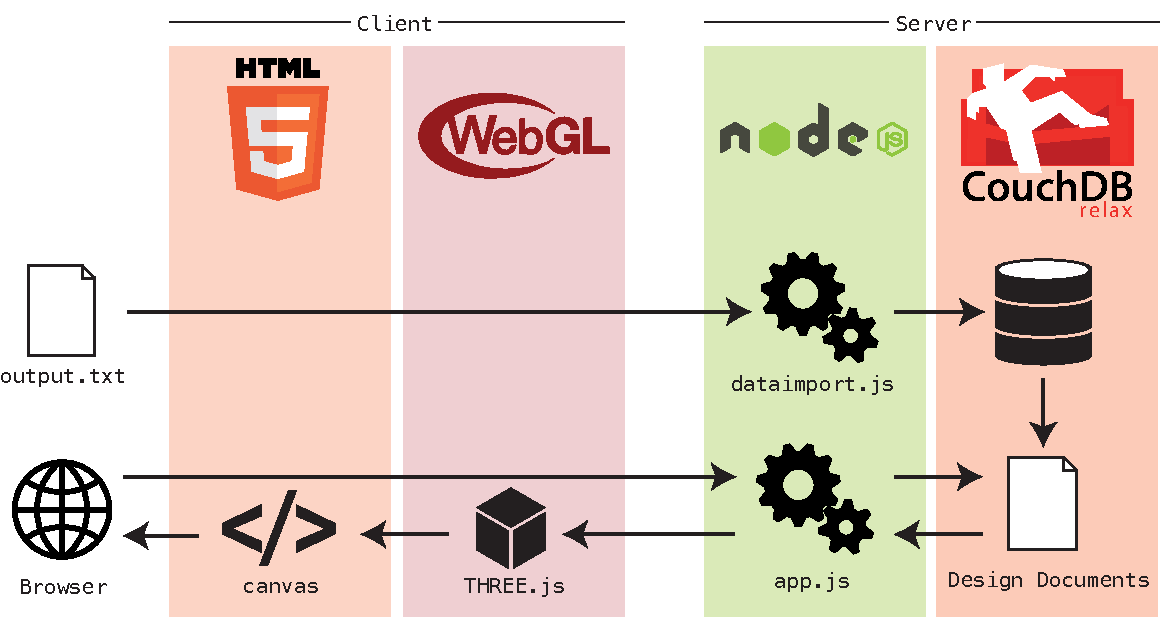
\includegraphics[width=\textwidth]{media/tec-stack.pdf}
\caption{Struktureller Aufbau von SumoViz3D}
\label{tecstack}
\end{figure}

In dieser Arbeit ist die Entwicklung der Software \emph{SumoViz3D} als Weiterentwicklung von Mustafa K. Isiks SumoViz beschrieben. SumoViz3D soll den Ansatz von SumoViz aufgreifen, aber die browserbasierte Darstellung um eine dreidimensionale Ansicht der Fu�g�ngersimulationsdaten erweitern. Zus�tzlich sollen Werte wie die Geschwindigkeit oder Dichte der Fu�g�nger ablesbar sein. Die Software soll kleinere Anpassungen am Aussehen der Szene erm�glichen und diese dabei m�glichst realistisch darstellen.

F�r SumoViz3D wird die bestehende serverseitige Architektur den Anforderungen entsprechend erweitert und die Client-Seite von Grund auf neu entwickelt. Die Ver�nderungen, die serverseitig durchgef�hrt werden m�ssen, passen lediglich die Ausgabe der Daten an, um die f�r die 3D-Darstellung ben�tigte Werte wie H�he, Typ des Hindernis oder Dichte der Fu�g�nger auszuliefern. Der Dateiimport \verb+dataimport.js+ wird um eine Funktionalit�t f�r das Importieren von Gruppendaten erweitert. 

In den folgenden Kapiteln werden die serverseitigen Ver�nderungen an der bestehenden SumoViz-Anwendung sowie die Neuentwicklung der Client-Seite beschrieben.





\chapter{Serverkomponenten: CouchDB und node.js} 
Apache CouchDB ist ein Datenbanksystem der \emph{Apache Software Foundation} das einen dokumentenorientieren Ansatz einsetzt. Im Gegensatz zu relationalen Datenbanken wird bei dokumentenorientieren Datenbanken kein festes Schema vorgegeben in dem die Datens�tze abgelegt werden. Stattdessen wird jeder Datensatz als Dokument mit beliebiger eigener Struktur in der Datenbank abgelegt. Jedes Dokument ist als JSON-Objekt repr�sentiert und hat mindestens ein Feld \verb+_id+ zur Identifikation. Der Zugriff auf die Daten erfolgt per HTTP-REST-Schnittstelle. Das bedeutet der Aufruf einer bestimmten URL liefert per HTTP die angeforderten Datens�tze zur�ck. �ber das HTTP-POST-Kommando k�nnen Daten in die Datenbank eingef�gt werden. \cite{ALS10}

Abfragen von einzelnen oder mehreren Datens�tzen werden \emph{Views} genannt. Views k�nnen in so geannten \emph{Design documents} gespeichert werden und sind dann f�r die Abfrage per HTTP-Request verf�gbar. CouchDB speichert die einzelnen Views zwischen, damit diese schneller verf�gbar sind. Zur Realisierung von Filtern und gezielten Abfragen verwendet CouchDB das \emph{MapReduce}-Verfahren, bei dem auf den Datenbestand nacheinander erst ein \emph{map}- und dann ein \emph{reduce}-Schritt ausgef�hrt wird. Diese Schritte werden durch JavaScript-Funktionen beschrieben und k�nnen komplexe Aufgaben auf den Daten ausf�hren. Solange der Datenbestand sich nicht ver�ndert hat, muss das Ergebnis des MapReduce nicht neu berechnet werden. Der map-Schritt wird f�r jedes Dokument der Datenbank ausgef�hrt und transformiert es in eine neue Struktur. Als R�ckgabe wird pro Datensatz kein, ein, oder mehrere Key-Value-Paare erwartet, die mittels \verb+emit(key,value)+ ausgegeben werden. Zus�tzlich k�nnen hier mittels if-Abfragen Filter implementiert werden.

Der reduce-Schritt ist optional und wird ausgef�hrt, wenn das Zwischenergebnis des map-Schritts gruppiert werden soll. Als Parameter wird ein Array mit den Keys und ein Array mit den Values des map-Schritts �bergeben. Auf diesen Arrays kann dann eine eigene Gruppierungsfunktion definiert werden. Bei gro�en Datens�tzen wird die reduce-Funktion f�r einzelne Abschnitte des Zwischenergebnisses aufgerufen und anschlie�end nochmal f�r die bereits reduzierten Teilergebnisse. Deshalb wird noch der Parameter \verb+rereduce+ �bergeben, der mitteilt, ob es sich um einen bereits reduzierten Datensatz handelt. Diese m�ssen dann meist nicht mehr reduziert sondern lediglich zusammengef�gt werden. Hintergrund dieses Verfahrens ist es auch extrem gro�e Datenmengen (in kleinen Schritten) verarbeiten zu k�nnen. \cite{Hol11}

% http://www.slideshare.net/okurow/couchdb-mapreduce-13321353
% MapReduce Views in CouchDB, Bradley Holt, O�Reilly, 2011 

Die zweite serverseitige Komponente ist \emph{node.js}, das aus Googles \emph{V8} JavaScript-Engine und einigen weiteren Komponenten besteht und damit die serverseitige Ausf�hrung von JavaScript-Code erm�glicht. Node.js ist sehr leistungsf�hig, da der JavaScript-Code vor der Ausf�hrung in Maschinensprache �bersetzt wird. Die Einbindung zus�tzlicher Komponenten ist bei node.js �ber Module m�glich, die �ber den Paketmanager \emph{npm (Node Packaged Modules)} installiert werden k�nnen. \cite{McL11} Auf Serverseite von SumoViz wird node.js f�r das Importieren (\verb+dataimport.js+) und Ausliefern (\verb+app.js+) der Daten eingesetzt.

\section{Importieren der Simulationsdaten}

Die Ergebnisse der Simulation werden in eine Textdatei geschrieben, die zur Verwendung mit SumoViz eingelesen und in der Datenbank abgelegt wird. Die Datens�tze sind zeilenweise in der Ausgangsdatei abgelegt und in Bl�cke unterteilt. Bl�cke innerhalb der Datei werden mit \verb+Begin+ und \verb+End+ sowie dem Blocknamen gekennzeichnet. Beispielsweise sind die Daten der Baugeometrie im Block \verb+Begin geometry+ angelegt. Die Ausgangsdatei enth�lt immer einen Block mit Parametern zur Simulation, die in SumoViz nicht verwendet werden, da die Parameter haupts�chlich f�r die Erstellung der Simulation, nicht aber f�r die Visualisierung n�tig sind.

F�r das Importieren der Daten in die \emph{CouchDB}-Datenbank exsistiert das node.js-Skript \verb+dataimport.js+. Es verarbeitet die Ausgangsdatei block- und zeilenweise und legt die Daten dann in der Datenbank ab. Das Skript verarbeitet nur die Bl�cke \verb+Geometry+, \verb+Data+ und \verb+Group Data+, alle anderen Inhalte der Ausgangsdatei werden ignoriert. F�r die Verbindung zur CouchDB wird das Modul \emph{cradle} verwendet. Zun�chst legt das Skript ein JSON-Array mit allen einzuf�genden Datens�tzen an, dieses wird dann mittels \emph{bulk insertion} in die Datenbank geschrieben. 



\subsection{Import der Fu�g�ngerdaten}

Durch Zeilen mit den Schl�sselw�rtern \verb+Begin Data+ und \verb+End Data+ ist innerhalb der Ausgabedatei ein Abschnitt mit den Fu�g�ngerpositionsdaten ausgezeichnet. Die Datens�tze enthalten einen Zeitstempel, eine Identifikationsnummer des Fu�g�ngers, Positionsdaten und Angaben zur Ebene auf der sich der Fu�g�nger befindet sowie zur Dichte. Pro Zeitpunkt und sichtbaren Fu�g�nger wird eine Zeile in der Ausgabedatei generiert. Die Werte des Datensatzes sind mit Leerzeichen getrennt und haben folgenden Aufbau:
\begin{table}[h]
\centering
\begin{tabular}{l||l|l|l|l|l|l|l}
& \textbf{timecode} & \textbf{pedid} & \textbf{x} & \textbf{y} & \textbf{z} & \textbf{level} & \textbf{density} \\
\hline
\hline
\textbf{Datentyp} & \verb+float+ & \verb+int+ & \verb+float+ & \verb+float+ & \verb+float+ & \verb+int+ & \verb+float+ \\
\hline
\textbf{Beispiel} & \verb+14.02+ & \verb+32+ & \verb+30.06+ & \verb+36.04+ & \verb+0.00+ & \verb+0+ & \verb+0.17+ \\
\end{tabular}
\label{tbl:tablelabel}
\caption{Struktur der Fu�g�ngerdaten}
\end{table}

\subsection{Import der Geometrie}

Der Block \verb+Geometry+ enth�lt eine Gliederung in unterschiedliche Stockwerke, gekennzeichnet mit \verb+begin floor+, gefolgt von einer H�henangabe zum jeweiligen Stockwerk. SumoViz und SumoViz3D unterst�tzen die Darstellung von Stockwerken nicht und ignorieren diese Daten deshalb. Dann folgen zeilenweise die einzelnen geometrischen Objekte. Beim Import werden nur Datens�tze im Format \verb+Polygon+ importiert. Es gibt zum Beispiel noch den Typ \verb+Image+ mit dem Grafiken �ber die Szene gelegt werden k�nnen. Dieser wird aber nicht unterst�tzt und daher ebenfalls ignoriert.

Ein Polygon besteht aus einer beliebigen Anzahl Koordinatenpaare $(x_i,y_i)$, die jeweils einen Eckpunkt des Polygons darstellen. Daher sollte die Mindestzahl an Eckpunkten $3$ sein. Eine H�henangabe ist optional, wird aber von einigen Geometrietypen beim rendern erwartet (vgl. Kapitel \ref{geo}). Die Struktur der Geometriedaten ist in Tabelle \ref{geotab} dargestellt.


\begin{table}[h]
\centering
\begin{tabular}{l||l|l|l|l|l|l|l}
& \textbf{format} & \textbf{x}$_0$ & \textbf{y}$_0$ &  \textbf{\ldots} & \textbf{name} & \textbf{type} & \textbf{height}\footnotemark \\
\hline
\hline
\textbf{Datentyp} & \verb+String+ & \verb+float+ & \verb+float+ &  \ldots & \verb+String+ & \verb+String+ & \verb+float+ \\
\hline
\textbf{Beispiel} & \verb+Polygon+ & \verb+40.39+ & \verb+42.69+ &  \ldots & \verb+o2+ & \verb+obstacle+ & \verb+3.5+ \\
\end{tabular}
\caption{Struktur der Geometriedaten}
\label{geotab}
\end{table}
\footnotetext{optional}

\subsection{Import der Gruppendaten}

F�r die Visualisierung der Gruppen in SumoViz3D wurde der Import f�r Gruppendaten im \verb+dataimport.js+-Skript hinzugef�gt. Gruppendaten sind nicht in allen Ausgabedateien angelegt, falls sie vorhanden sind ist der Block entsprechend mit \verb+Group Data+ gekennzeichnet und in der Visualisierung steht die Einf�rbung nach Gruppen zur Verf�gung (siehe Kapitel \ref{colorgroups}). Ein Datensatz beinhaltet die Zugeh�rigkeit eines Fu�g�ngers zu einer Gruppe. Einzelne Gruppen werden dabei implizit durch die Verwendung der jeweiligen Gruppen-ID erzeugt. Zus�tzlich ist noch die Gruppengr��e mit angegeben (vgl. Tabelle \ref{grouptab}). Dieser Wert ist aber redundant, da die Gruppengr��e auch mittels Summenfunktion berechnet werden kann und wird deshalb nicht mit importiert.

\begin{table}[h]
\centering
\begin{tabular}{l||l|l|l}
& \textbf{pedid} & \textbf{groupid} & \textbf{size} \\
\hline
\hline
\textbf{Datentyp} & \verb+int+ & \verb+int+ & \verb+int+ \\
\hline
\textbf{Beispiel} & \verb+241+ & \verb+32+ & \verb+3+  \\
\end{tabular}
\caption{Struktur der Gruppendaten}
\label{grouptab}
\end{table}



\section{Ausgabe der Simulationsdaten}
\label{chapmapreduce}
Alle Daten der Visualisierung muss der Client vom Server nachladen. Dabei handelt es sich um den Namen der Animation, Positionsdaten der Fu�g�nger, die bauliche Geometrie und die Gruppendaten. Jede dieser Abfragen hat eine eigene URL als Endpunkt. Node.js agiert als Webserver, verarbeitet die Anfragen und liefert entsprechend die Daten aus CouchDB aus. Die Aufbereitung der Daten findet ausschlie�lich in der Datenbank mittels der MapReduce-Funktionen statt. Nach dem Laden der Daten im JSON-Format werden diese im Client geparst und stehen dann als JavaScript-Objekt zur Verf�gung.

\subsection{Ausgabe der Fu�g�ngerdaten}

F�r SumoViz wurden lediglich die x-y-Koordinaten der Fu�g�nger nach Zeitpunkt gruppiert und als JSON-Array ausgegeben. Die Visualisierung in SumoViz3D ben�tigt aber noch weitere Daten, weshalb das Datenformat umstrukturiert und erweitert werden musste. Die Fu�g�nger-ID (\verb+pedid+) ist notwendig um die Gruppenzuordnung zu erhalten und  die Positionsdaten eines Fu�g�ngers zu fr�heren oder sp�teren Zeitpunkten zu bestimmen. Das ist f�r die Bestimmung der Geschwindigkeit und Bewegungsrichtung notwendig und kann bei zuk�nftigen Erweiterungen wie dem Tracing einzelner Fu�g�nger n�tzlich sein (vgl. Kapitel \ref{erweiterungen}). Zus�tzlich wird noch die Dichte (\verb+density+) pro Fu�g�nger pro Zeitpunkt ausgeliefert. Diese Daten waren auch bisher schon gespeichert und wurden nur noch nicht mitausgeliefert. Das Format der Dokumente in CouchDB bleibt unver�ndert und bestehende Datens�tze m�ssen nicht neu importiert werden. Lediglich die MapReduce-Funktionen der Design Documents wurden angepasst.


Die map-Funktion f�r die Fu�g�ngerdaten (siehe Listing \ref{mapfkt}) von SumoViz wurde nur geringf�gig erweitert, so dass im Value-Array nun neben der Position auch die ID und die Dichte ausgegeben werden. 
\begin{lstlisting}[caption=CouchDB map-Funktion f�r Fu�g�ngerdaten,label=mapfkt]
function(doc) {
    if (doc.pedid !== undefined) {
        emit(doc.time, [doc.x,doc.y,doc.density,doc.pedid]);
    }
}
\end{lstlisting}
Die ausgegebenen Key-Value-Paare werden mit einer komplett neu geschreibenen reduce-Funktion gruppiert (siehe Listing \ref{reducefkt}). Die Werte werden nicht mehr in einer Array gespeichert sondern in einem Objekt pro Zeitpunkt (Listing \ref{reducefkt}, Zeile \verb+12+). In diesem Objekt wird f�r jeden Fu�g�nger ein Key mit entsprechender Fu�g�nger-ID (\verb+values[i][3]+) und einem Array aus Positions- (\verb+values[i][0]+ und \verb+values[i][1]+) und Dichtedaten (\verb+values[i][2]+) als Value angelegt (Listing \ref{reducefkt}, Zeile \verb+13+). Das erm�glicht den direkten Zugriff auf Daten einer bestimmten Fu�g�nger-ID mit dem Aufruf \verb+pedestrianData[zeitpunkt][id]+ ohne die Anwendung einer linearen Suche durch alle Werte des Zeitpunktes nach der gesuchten ID.

Wird die Bearbeitung der Daten auf Grund der Gr��e aufgeteilt, so bekommt die reduce-Funktion im rereduce-Fall (Listing \ref{reducefkt}, Zeile \verb+2+) ein Array aus Objekten, die je einen Teil der schon gruppierten Fu�g�ngerdaten des jeweiligen Zeitpunkts enthalten. Dieses Array mit Objekten muss zu einem einzelnen Objekt (\verb+values[0]+) zusammengef�gt werden und ergibt dann das fertige Datenobjekt f�r den entsprechenden Zeitpunkt. Eine Kollision der Keys beim Zusammenf�gen der Objekte ist ausgeschlossen, da die Keys den IDs der Fu�g�nger entsprechen, die zu jedem Zeitpunkt einmalig sind.

\clearpage

\begin{lstlisting}[caption=CouchDB reduce-Funktion f�r Fu�g�ngerdaten,label=reducefkt]
function(keys, values, rereduce) {
    if(rereduce) {
        for (i=1;i<values.length;i++) {
            for (var key in values[i]) {
                values[0][key] = values[i][key];
            }
        }
        return values[0];
    } else {
        var sortedValues = {};
        for(var i = 0; i < values.length; i++) {
            sortedValues[values[i][3]] = 
                            [values[i][0],values[i][1],values[i][2]];
        }
        return sortedValues;
    }
}
\end{lstlisting}

Ein beispielhaftes Datenobjekt der Fu�g�ngerdaten f�r einen bestimmten Zeitpunkt der Simulation kann wie folgt aussehen:

\verb+    {"0":[40.23,40.05,0],"1":[40.69,37.64,0],"2":[40.92,36.44,0],...}+

\subsection{Ausgabe der Geometrie- und Gruppendaten}

Die Ausgabe der Geometriedaten ben�tigt keine Gruppierung und dementsprechend nur eine map-Funktion, die pro Geoemetrie-Objekt ein JSON-Objekt ausgibt, das die x-y-Koordinaten in Form eines Arrays und Typ, Name und H�he als Properties darstellt. Ein entsprechendes JSON-Objekt kann zum Beispiel so aussehen:

\verb+    {geometry: [[64.42, 33.3], [61.2, 35.7], ...],+\\
\verb+            "height": 3.5, "name": "plant0", "type": "obstacle"}+


Das Ursprungsformat der Gruppendaten wird nach dem Key, der Gruppen-ID, gruppiert. Pro Gruppen-ID wird dann ein Array mit den in der Gruppe enthaltenen Fu�g�nger-IDs ausgegeben. Die reduce-Funktion muss lediglich das schon gruppierte values-Array ausgeben, bzw. im rereduce-Fall werden die einzelnen value-Arrays zu einem einzigen Array (\verb+values[0]+) verbunden (vgl. Listing \ref{groupreducefkt} Zeile \verb+4+). Die Gruppen-ID wird f�r die Darstellung im Client nicht mehr ben�tigt.

\begin{lstlisting}[caption=CouchDB reduce-Funktion f�r Gruppendaten,label=groupreducefkt]
function (keys,values,rereduce) {
    if (!rereduce) return values;
    else {
        for (i=1;i<values.length;i++) values[0].concat(values[i]);
        return values[0];
    }
}
\end{lstlisting}


\chapter{Clientseitige Entwicklung von SumoViz3D}

Clientseitig verwendet SumoViz3D die THREE.js-Bibliothek um die Simulationsdaten in WebGL darzustellen. Mit der JavaScript-Bibliothek \emph{jQuery UI}, HTML und CSS wird die Bedienoberfl�che erstellt.

\section{Das Interface von SumoViz3D}

Das canvas-Element zur Darstellung der Simulation wird in der vollen Browsergr��e dargestellt, alle anderen Elemente werden als Overlay aus HTML-Elementen gestaltet. Dabei werden viele Bestandteile mittels jQuery UI umgesetzt. Dieses JavaScript-Framework macht es m�glich Interface-Elemente wie Buttons und Dialogboxen einfach und cross-browserkompatibel anzulegen. \cite{jQu}

\begin{figure}[h]
\begin{center}
\includegraphics[width=\textwidth]{media/screenshot.png}
\caption{Screenshot des SumoViz3D-Interfaces}
\label{screenshot}
\end{center}
\end{figure}

Die Toolbar (Abbildung \ref{screenshot} \circled{1}) erm�glicht die Steuerung des Ablaufs der Animation. Mit dem Play/Pause-Button kann die Animation abgespielt und angehalten werden. Der aktuelle Stand der Visualisierung kann mittels des Sliders ver�ndert werden. Zus�tzlich wird noch angezeigt, welcher Simulationsschritt aktuell dargestellt wird. �ber die Pfeil-Buttons l�sst sich schrittweise durch die Simulation navigieren. �ber den Einstellungs-Button wird ein Dialog aufgerufen, �ber den globale Modifikationen an der Szene vorgenommen werden k�nnen (Abbildung \ref{screenshot} \circled{2}). Zus�tzlich lassen sich durch einen Kontextklick auf die Geometrieobjekte die objektbezogenen Modifikationen aufrufen (Abbildung \ref{screenshot} \circled{3}).

Die THREE.js-Erweiterung \emph{Stats} (Abbildung \ref{screenshot} \circled{4}) zeigt die aktuelle Framerate mit der die Szene gezeichnet wird. Dazu wird im Aufruf der Zeichenmethode (siehe Kapitel \ref{raf}) zus�tzlich noch ein Aufruf von \verb+stats.update()+ platziert, der dann die Zeit zwischen dem aktuellen Aufruf und dem letzten bestimmt und so die Framerate errechnet. \cite{MrD} Durch einen Klick auf das Modul l�sst sich auch die ben�tigte Ausf�hrungszeit der Zeichenmethode in Millisekunden anzeigen. In Klammern sind Minimum und Maximum angegeben.

Die Legende (Abbildung \ref{screenshot} \circled{5}) passt sich den Ansichtsoptionen an und zeigt f�r die Einf�rbung nach Geschwindigkeit und Dichte die entsprechende Farbkodierung der Fu�g�nger an. Wenn das Gitternetz sichtbar ist, wird der Abstand der Gitternetzlinien in Metern angezeigt.



\section{Darstellung der Geometrie}
\label{geo}
Die geometrischen Objekte zur Darstellung der Umgebung enthalten in ihrer Datenstruktur die Beschreibung ihres Grundrisses in Form von x-y-Koordinaten, eine H�henangabe, den Namen und ein Typen-Feld. F�r die Darstellung ma�geblich entscheidend ist der Inhalt des Typen-Felds. Es entscheidet, welche Renderingroutine verwendet wird. Folgende Typen werden von SumoViz3D unterschieden: \verb+geometry+, \verb+obstacle+, \verb+wall+. Zudem gibt es noch eine vierte Renderingroutine f�r alle anderen Typen unter die vor allem \verb+source+, \verb+target+ und \verb+field+ fallen.

Die Berechnung der Geometrie erfolgt beim Laden der Simulation und muss nur einmalig ausgef�hrt werden. Dazu wird die Methode \verb+drawGeometry+ definiert. Wird die Geometrie w�hrend der Laufzeit ver�ndert, wird diese Methode erneut aufgerufen (siehe Kapitel \ref{recallgeo}).
 
\subsection{Skalierung der Geometrie}

Die darzustellende Geometrie kann extrem unterschiedliche Dimensionen haben. Trotzdem soll nach dem Laden der Szene die Kamera so positioniert sein, dass ein �berblick �ber die gesamte Szene m�glich ist.

\begin{wrapfigure}{r}{0.5\textwidth}
\vspace{-5pt}
  \includegraphics[width=0.5\textwidth]{media/zfighting.png}
  \caption{Z-Fighting zwischen Grundebene und Feldern bei gro�er Kameradistanz}
  \label{fig:zfighter}
\vspace{-5pt}
\end{wrapfigure}


Erster Ansatz zur L�sung war es, die Kameradistanz entsprechend der Gr��e der Szene mitzuskalieren. Jedoch trat hierbei \emph{Z-Fighting} auf. Ein bekanntes Problem aus dem 3D-Bereich, bei dem durch Rundungsfehler Fehler in der Darstellung auftreten. Bei einer hohen Distanz zwischen Kamera und Objekten ist der relative Abstand der Objekte zueinander sehr gering. Durch mangelnde Genauigkeit in der Speicherung der Tiefenwerte zweier Objekte kann nicht mehr entschieden werden, welches Objekt vor dem jeweils anderen liegt. Objekte die eigentlich verdeckt sein m�ssten, flimmern an manchen Stellen durch die Oberfl�che hindurch (vgl. Abbildung \ref{fig:zfighter}).

Zur L�sung des Problems wird nun die Kameradistanz f�r jede Szene unver�ndert gelassen und die Geometrie- und Fu�g�ngerobjekte entsprechend der Gr��e der Grundebene (\verb+geometrySize+) skaliert. Dazu wird ein Skalierungsfaktor \verb+globalScale+ wie folgt berechnet:

\verb|    globalScale = 50/((geometrySize.x+geometrySize.y)/2);|

Der Faktor 50 wurde empirisch bestimmt und an die Einstellungen der Kamera angepasst. Jedes Objekt wird mit dem Skalierungsfaktor multipliziert und entsprechend vergr��ert oder verkleinert. Einige weitere Vorteile ergeben sich aus diesem Vorgehen: Die Lichter m�ssen nicht an die Szenengr��e angepasst werden um diese vollst�ndig auszuleuchten, denn absolut gesehen hat jede Szene exakt die gleiche Gr��e. Selbiges gilt f�r die Steuerung der Kamera (vgl. Kapitel \ref{controls}) die nicht auf die Szenengr��e angepasst werden muss.

\subsection{Darstellung der Grundebene und des Gitternetzes}
In den Geometriedaten befindet sich immer ein Element vom Typ \verb+geometry+, das eine rechteckige Grundfl�che definiert die alle Objekte enth�lt. Diese Fl�che wird orthogonal zur y-Achse des WebGL-Koordinatensystems eingezeichnet und beginnt im Ursprung. Auf dieser Grundebene wird ein Gitternetz eingezeichnet, das zwei Zwecke erf�llt: Einerseits helfen die Linien, die auf den Fluchtpunkt zulaufen bei der Tiefenwahrnehmung. Andererseits lassen sich mit dem in der Legende angegebenen ``grid pitch'' die Gr��enverh�ltnisse besser beurteilen. Dieser Wert gibt den Abstand zweier benachbarter Gitternetzlinien in Metern an. Eine Ma�stabangabe wie in Landkarten ist auf Grund der perspektivischen Abbildung nicht m�glich.


\subsection{Darstellung von Objekten des Typ ``obstacle''}
Geometrie vom Typ \verb+obstacle+ sind bauliche Hindernisse wie Geb�ude oder auch B�ume und Pflanzen. Diese m�ssen von den Fu�g�ngern umgangen werden. F�r die Darstellung dieser Hindernisse wird ein Polygon aus den x-y-Koordinaten erzeugt. Mit einer \verb+ExtrudeGeometry+ wird aus dem flachen Polygon dann ein dreidemensionales Objekt erzeugt (vgl. Abbildung \ref{obstacle}). Hierf�r wird die beim Objekt gespeicherte H�henangabe ben�tigt.



\begin{figure}[ht]
\begin{minipage}[b]{0.48\linewidth}
\centering
\includegraphics[width=\textwidth]{media/obstacle.png}
\caption{Darstellung von normalen Objekten (blau)}
\label{obstacle}
\end{minipage}
\hspace{0.3cm}
\begin{minipage}[b]{0.48\linewidth}
\centering
\includegraphics[width=\textwidth]{media/tree.png}
\caption{Darstellung von B�umen mittles COLLADA-Modell}
\label{tree}
\end{minipage}
\end{figure}


B�ume und Pflanzen werden gesondert dargestellt. Die Erkennung davon erfolgt �ber den Namen des Objekts, da diese ebenfalls den Typ ``obstacle'' haben. Ein entsprechendes Objekt kann beispielsweise \verb+tree0+ benannt sein. Enth�lt also ein Objektname \verb+tree+ oder \verb+plant+ wird die Darstellung angepasst. Dazu sind in SumoViz3D externe Modelle eines Baums und eines Buschs hinterlegt, wie in Abbildung \ref{tree} zu sehen. THREE.js bietet verschiedene Erweiterungen zum importieren von externen 3D-Modellen in unterschiedlichen Formaten. SumoViz3D verwendet den \verb+ColladaLoader+, der Modelle im \emph{COLLADA}-Format importieren kann. \emph{COLLADA (COLLAborative Design Activity)} ist ein offenes XML-Format f�r die Speicherung von Modellen, Texturen und ganzen Szenen. Das Format wird wie WebGL auch von der Khronos Group verwaltet und kann in vielen 3D-Programmen im- und exportiert werden. \cite{COL}

Das Baum- bzw. Busch-Modell wird mittels des Loaders aus der Datei geladen und geparst. Danach steht es als normales 3D-Objekt zur Verf�gung und kann skaliert und positioniert werden. Um die Ladezeit gering zu halten, wurden die Modelle mit sehr wenigen Vertices angelegt und mit einfachen Texturen versehen. Die Dateigr��e des Baum-Modells mit Grafiktextur betr�gt etwa 50 Kilobytes. Komplexere Modelle k�nnten mehrere Megabytes gro� sein und das Nachladen �ber die Internetverbindung w�rde zu lange dauern.

%https://collada.org/mediawiki/index.php/COLLADA_-_Digital_Asset_and_FX_Exchange_Schema


\subsection{Darstellung von Objekten des Typ ``wall''}

\begin{wrapfigure}{r}{0.4\textwidth}
  \includegraphics[width=0.4\textwidth]{media/wall.png}
  \caption{Darstellung von W�nden ohne Textur}
  \label{wall}
\end{wrapfigure}

W�nde sind als Pfad definiert. Die einzelnen Koordinaten werden linear verbunden und ergeben so die Grundlinie der Wand. Um in der 3D-Darstellung realistischer zu wirken sollen die W�nde auch noch eine Dicke erhalten. Dazu wird aus jeweils zwei benachbarten Pfadpunkten und den selben Punkten, die aber in der H�he verschoben wurden, ein Rechteck gebildet. Die H�he der Wand stammt dabei auch aus den importierten Ursprungsdaten. Dieses Rechteck wird wieder mit \verb+ExtrudeGeometry+ um die Dicke der Wand zu einem Quader ausgedehnt. Da eine Wand mehr als zwei Pfadpunkte haben kann, werden die entstandenen Quader dann wieder zu einem Objekt zusammen gef�gt und angezeigt (vgl. Abbildung \ref{wall}).


\subsection{Darstellung anderer Objekte}

\begin{wrapfigure}{r}{0.4\textwidth}
  \includegraphics[width=0.4\textwidth]{media/field.png}
  \caption{Darstellung von Quelle, Ziel und anderen Feldern (rot)}
  \label{field}
\end{wrapfigure}
Hat die Geometrie einen anderen Typ, so wird sie als flaches, halbtransparentes Polygon auf der Grundebene dargestellt (vgl. Abbildung \ref{field}). Alle Szenen haben mindestens ein Objekt vom Typ \verb+source+ das der Startpunkt der Fu�g�nger ist. Entsprechend exsistiert \verb+target+, welches das Ziel der Fu�g�nger darstellt. Pro Szene k�nnen auch mehrere Start- und Zielfelder vorhanden sein. Der Typ \verb+field+ wird ebenso dargestellt und markiert Bereiche, die beispielsweise besondere Auswirkungen wie Verlangsamung oder Beschleunigung auf die Fu�g�nger haben. Aber auch v�llig unbekannte Geometrietypen k�nnen in diesem Fallback zumindest grundlegend angezeigt werden.


\subsection{Ver�nderung w�hrend der Laufzeit}
\label{settings}
Eigentlich ist die Geometrie w�hrend der gesamten Zeit unver�ndert und wird deshalb nur initial berechnet. SumoViz3D erm�glicht dem Betrachter zus�tzlich das Erscheinungsbild der Szene anzupassen und so ein realistischere Darstellung zu erzeugen. Folgende Modifikationen an der Geometrie sind dem Benutzer w�hrend der Laufzeit m�glich:

\clearpage

\textbf{Globale Modifikationen:}
\begin{itemize}
    \item Darstellung der Fu�g�nger als Partikel oder 3D-Modelle
    
    \item Das Gitternetz der Grundebene l�sst sich ein- und ausblenden.
    
    \item Die Textur der Grundebene kann ver�ndert werden. Es steht eine Auswahl verschiedener Grafiktexturen, wie beispielsweise Wiese oder Erde, zur Verf�gung.

    \item Es kann eine Grafiktextur f�r alle W�nde ausgew�hlt werden. Hier steht ebenfalls eine Vorauswahl zur Verf�gung.
\end{itemize}

\textbf{Objektbezogene Modifikationen:}
\begin{itemize}
    \item Einzelne Objekte der Szene lassen sich entfernen.

    \item Alle Objekte, au�er B�ume und B�sche, lassen sich individuell einf�rben.

    \item Objekte vom Typ \verb+obstacle+ lassen sich zu B�umen oder B�schen konvertieren. Dazu wird vor den bestehenden Objektnamen der Prefix \verb+tree_+ oder \verb+plant_+ gesetzt. 
\end{itemize}
Globale Modifikationen k�nnen �ber das Einstellungsmen� in der Toolbar vorgenommen werden. F�r objektbezogene Modifikationen muss ein entsprechendes Objekt mit einem Kontextklick ausgew�hlt werden. Um zu erkennen welches Objekt durch den Kontextklick ausgew�hlt wurde ist eine Berechnung n�tig, welche die 2D-Koordinaten des JavaScript-Events \verb+contextmenu+ auf die 3D-Szene umgerechnet. Die x- und y-Koordinaten des Klicks werden in das WebGL-Koordinatensystem (vgl. Kapitel \ref{tecandfunc}) konvertiert und f�r die z-Achse wird ein fester Wert verwendet. Dann wird ein Strahl ausgehend von der Kameraposition in Richtung des Klickpunkts berechnet und die durchquerten Objekte ermittelt. Das erste dieser Objekte ist das vom Benutzer ausgew�hlte, da die sp�ter durchkreuzten Objekte verdeckt und damit f�r den Nutzer nicht sichtbar sind.


\subsubsection{Speichern der Einstellungen}
\label{recallgeo}

Die Modifikationen, die durch den Benutzer vergenommen wurden, sollen persistent gespeichert werden. Zu diesem Zweck wird die \emph{WebStorage}-API, die mit HTML5 spezifiziert wurde, verwendet. Es handelt sich dabei um lokalen Speicher in Form von Key-/Value-Paaren. Einschr�nkend ist hierbei, dass nur Strings gespeichert werden k�nnen. Um andere Datentypen zu speichern, k�nnen diese beispielsweise im JSON-Format hinterlegt werden. F�r die Gr��e des Speichers schl�gt das W3C 5 Megabytes vor. \cite{W3s} Zugriff auf den Speicher erfolgt �ber das \verb+localStorage+-Objekt mittels der Methoden \verb+setValue(key, value)+ und \verb+getValue(key)+ oder alternativ �ber die Punktschreibweise \verb+localStorage.key+ oder assoziative Arrays \verb+localStorage["key"]+. �nderungen im Speicher m�ssen nicht mehr explizit gespeichert werden und sind �ber die Session hinaus beliebig lange verf�gbar. Mit \verb+localStorage.clear()+ l�sst sich der Inhalt des Speichers l�schen. \cite{diveInto}

Alle Ver�nderungen an den in Kapitel \ref{settings} beschriebenen Einstellungen werden pro Simulations-Datensatz im lokalen Speicher abgelegt. Die vorgenommenen �nderungen sind sofort, ohne explizites speichern, persistent und lokal gesichert und damit nicht f�r andere Nutzer sichtbar. Nach dem Laden der Szene wird gepr�ft ob f�r die jeweiligen Simulationsdaten bereits Einstellungen hinterlegt wurden und diese gegebenenfalls geladen und angewendet.

Zum Ablegen der globalen Modifikationen wird das Schl�sselformat \verb+animationName_setting+ verwendet. Zudem werden unter dem Schl�ssel \verb+animationName_objectSettings+ die objektbezogenen Anpassungen in einem Array gespeichert. Die Reihenfolge der Geometrieobjekte, wie sie aus der Datenbank ausgegeben werden, wird zugleich zur Identifikation der Objekte verwendet. An der jeweiligen Array-Position werden die Anpassungen f�r das entsprechende Objekt gespeichert. Bleibt das Objekt unver�ndert, wird der Wert \verb+null+ eingetragen.

In Listing \ref{savejson} wird ein beispielhaftes JSON-Objekt zur Speicherung der Ver�nderungen an der Animation \verb+out_aStern+ abgebildet. 
\begin{lstlisting}[caption=Beispielhaftes JSON-Objekt zur Speicherung der �nderungen,label={savejson}]
{
    "out_aStern_showGrid": "no",
    "out_aStern_floorTexture": "textures/gray.jpg",
    "out_aStern_pedestrianColoring": "density",
    "out_aStern_objectSettings": [
        {"color": {"r": 1.00, "g": 0.00, "b": 0.00}},
        null,
        {"convert": "tree_obstacle0"}
    ]
}
\end{lstlisting}

In diesem Beispiel wurde das Gitternetz ausgeblendet (Zeile \verb+2+) und auf der Grundebene eine Grafiktextur aus der Datei \verb+textures/gray.jpg+ geladen  (Zeile \verb+3+). Die Einf�rbung der Fu�g�nger erfolgt nach der Dichte (Zeile \verb+4+). Au�erdem wurden zwei objektbezogene Modifkationen durchgef�hrt. Das Objekt mit der ID 0 wurde rot eingef�rbt (Zeile \verb+6+) und das Objekt mit der ID 2 wurde in einen Baum konvertiert (Zeile \verb+8+).

%https://developer.mozilla.org/en-US/docs/DOM/Storage?redirectlocale=en-US&redirectslug=DOM%3AStorage 
% http://www.w3.org/TR/webstorage/
% http://diveintohtml5.info/storage.html



%http://www.nczonline.net/blog/2011/05/03/better-javascript-animations-with-requestanimationframe/
%http://stackoverflow.com/questions/729921/settimeout-or-setinterval


Um Animationen in JavaScript auszuführen wurden die Funktionen \verb+setTimeout(function,delay)+ oder \verb+setInterval(function,interval)+ verwendet. Diese rufen dann in einem festgelegten Rhythmus eine Funktion auf, die inkrementell die Animation ausführt. Während \verb+setInterval+ nur einmalig aufgerufen wird und dann von alleine die Funktion im angegebenen Intervall aufruft, muss \verb+setTimeout+ nach der Ausführung des Animationsschritts erneut rekursiv aufgerufen werden. Jedoch gibt es einige Nachteile mit der Verwendung dieser Methoden. Die 



\section{Steuerung der Kamera}

\label{controls}
SumoViz3D verwendet eine perspektivische Kamera mit einem festeingestellten Sichtfeld von $45^\circ$. Die Positionierung und Ausrichtung der Kamera ist, mit einigen Einschr�nkungen, dem Nutzer �berlassen. W�hrend der Visualisierung k�nnen Kameraposition und -ausrichtung ver�ndert werden. Dazu wurde die Klasse \verb+SphereControls+ angelegt. Im Konstruktor der Klasse wird das Kamera-Objekt �bergeben, dessen Position manipuliert werden soll und das DOM-Element auf dem die Benutzereingaben erfolgen, in diesem Fall also das canvas-Element. Damit werden nur Eingaben die direkt auf dem canvas-Element erfolgen verarbeitet. Eingaben auf den HTML-Overlay-Elementen wie der Toolbar oder Dialogen werden f�r die Kamerasteuerung ignoriert. Event-Listener die auf Tastatur- und Mauseingaben reagieren werden mittels \verb+addEventListener+ an das canvas-Element angef�gt. \cite{Fla06}

\begin{wrapfigure}{r}{0.5\textwidth}
\vspace{-7pt}
  \begin{center}
    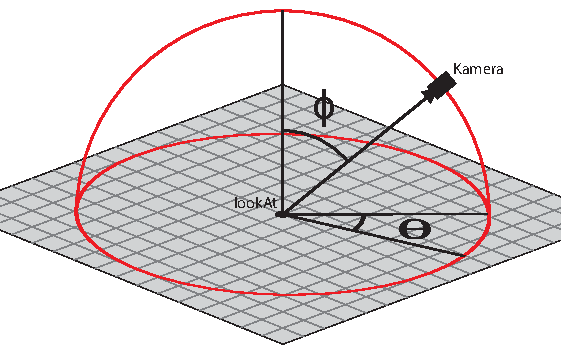
\includegraphics[width=0.5\textwidth]{media/camera.pdf}
  \end{center}
  \caption{Kameraposition}
  \label{cameramodel}
  
  \vspace{-7pt}
\end{wrapfigure}




Zur Ausrichtung der Kamera wird der Punkt \verb+lookAt+ definiert, auf den die Kamera stets ausgerichtet ist. Dieser Punkt liegt immer in der Grundebene der dargestellten Geometrie und kann dort bewegt werden. Die Kamera kann sich halbkugelf�rmig um diesen Punkt herum bewegen, aber dabei nicht unterhalb der Grundebene bewegt werden. Zur Berechnung der Position der Kamera sind neben der Position des \verb+lookAt+-Punktes noch der Radius $r$ der Kugel, der Neigungswinkel $\theta$ und der Drehwinkel $\phi$ notwendig. Mit folgenden Formeln lassen sich die Positionskoordinaten wie folgt berechnen: \cite{Gub09}

\vspace{3 mm}

\begin{tabular}{lll}
$x$ & $=$ & $lookAt.x + r \cdot \sin \theta \cdot \cos \phi$ \\
$y$ & $=$ & $lookAt.z + r \cdot \cos \theta$ \\
$z$ & $=$ & $lookAt.y + r \cdot \sin \theta \cdot \sin \phi \qquad (0 \le \theta \le \pi \ \wedge 0 \le \phi < 2 \pi)$
\end{tabular}

\vspace{3 mm}

In der Animations-Schleife wird die \verb+update+-Methode der Steuerung aufgerufen. Ist ein \verb+keydown+- aber noch kein \verb+keyup+-Event auf einer der Cursor-Tasten ausgel�st, so ist diese Cursor-Taste gerade gedr�ckt und die Position des \verb+lookAt+-Punkts wird in entsprechender Richtung ver�ndert. Die Richtung der Bewegung muss aber relativ zu aktuellen Drehung der Kamera erfolgen. Dazu wird der Vektor zwischen Kameraposition und \verb+lookAt+-Punkt berechnet. Von diesem Vektor wird die y-Komponente auf $0$ gesetzt, damit liegt er auf der Grundebene. Dann wird der Vektor (bzw. ein orthogonaler Verktor) normiert und beim dr�cken der Cursor-Tasten auf den \verb+lookAt+-Punkt addiert oder von diesem subtrahiert. 

Folgende Event-Listener sind zur Steuerung der Visualisierung auf das canvas-Element gelegt. Solange der Event-Listener ausgel�st ist wird mit jedem Aufruf der \verb+update+-Methode entsprechende Varaible(n) modifiziert: 

\clearpage

\begin{table}[h]
\centering
\begin{tabular}{lll}
\textbf{EventListener} & \textbf{modifizierte Variable} &\textbf{Funktionalit�t} \\
\hline
\verb+keydown+                     & \verb+lookAt+ & Bewegen  \\
\verb+mousedown+ + \verb+mousemove+       & $\theta$ und $\phi$ & Kamera drehen/neigen \\
\verb+mousewheel+\footnotemark & $r$ & Zoomen \\
\verb+contextmenu+             & $-$ &   Objekte anpassen  \\

\end{tabular}
\caption{Event-Listener und zur Steuerung modifizierte Variablen}
\end{table}

\footnotetext{In Firefox wird das Event DOMMouseScroll verwendet}
\vspace{3 mm}

F�r das Drehen und Neigen der Kamera wird die Distanz zwischen dem Punkt, an dem das \verb+mousedown+-Event ausgel�st wurde und der aktuellen Mauscursorposition berechnet. Die horizontale Distanz wird auf den Drehwinkel $\phi$ addiert und bewegt die Kamera im mathematischen Drehsinn auf der Kugeloberfl�che. Wird die Maus nach links gezogen, so hat die Distanz einen negativen Wert und wird vom Drehwinkel subtrahiert, was eine Bewegung gegen den mathematischen Drehsinn zur Folge hat. Die vertikale Distanz wird vom Neigungswinkel $\theta$ subtrahiert, da dieser der y-Achse her aufgespannt wird (vgl. Abbildung \ref{cameramodel}). Au�erdem wird verhindert das $\theta > \frac{\pi}{2}$ wird, um stets �ber der Grundebene zu bleiben.
\section{Darstellung der Fu�g�ngerdaten}

F�r die Darstellung vieler kleiner Elemente oder gibt es in der Computergrafik sogenante Partikelsysteme. Haupteinsatzzweck ist die Berechnung von Effekten wie Feuer, Rauch, Nebel oder Wasser. Ein Partikelsystem besteht aus einer gro�en Menge einzelner Partikel, von denen jeder eigene Eigenschaften haben kann. Der Vorteil der Verwendung eines Partikelsystems gegen�ber einzelnen Objekten ist die Minimierung der Objektanzahl. Ein Partikelsystem ist technisch nur ein einziges Objekt. Jeder Partikel wird als Vertex dieses Objekts an die Grafikkarte �bergeben. ...

Zur Darstellung wird das \verb+ParticleBasicMaterial+ verwendet. 
%http://mrdoob.github.com/three.js/docs/50/#ParticleBasicMaterial
Billboard

\subsection{Einf�rbung der Fu�g�ngerobjekte}
Als Billboard wird die Grafik einer wei�en Kugel mit Schatten verwendet. Darauf wird die zum jeweiligen Vertex gespeicherte Farbe multipliziert. Die dunklen Fl�chen bleiben dabei dunkel, die hellen Fl�chen werden eingef�rbt. So lassen sich verschiedene Daten visualisieren. SumoViz3D hat folgende Einf�rbungsm�glichkeiten zur Verf�gung:

\subsubsection{Einf�rbung nach Dichte}


Standardeinstellung ist die Einf�rbung nach Dichte. Pro Zeitpunkt und Fu�g�nger sind diese Daten schon in der Ausgabedatei gespeichert und m�ssen nicht mehr berechnet werden. Der Wertebereich ist mit $0.0 \le density \le 1.0$ definiert. Zur Farbgebung der Fu�g�nger ist die Verwendung des HSV-Farbraums geeignet zudem THREE.js die Methode \verb+setHSV(h,s,v)+ implementiert. Der Farbwert wird beim HSV-Farbraum �ber den Farbton $H$ (engl. \emph{hue}), die Farbs�ttigung $S$ (engl. \emph{saturation}) und den Hellwert $V$ (engl. \emph{value}) bestimmt. W�hrend $S$ und $V$ als Prozentwerte angegeben werden, wird f�r $H$ eine Farbwinkelangabe auf dem Farbkreis verwendet.

Bild: Color cone(CC-BY-SA-3.0 )

F�r die Dichte soll der Farbton zwischen gr�n ($H=105^\circ$) f�r einen Wert von $0.0$ und rot ($H=0^\circ$) f�r den Maximalwert von $1.0$ variieren. S�ttigung und Hellwert bleiben unver�ndert.
\begin{verb}
    particles.colors[i].setHSV(105-105*density,1,1);
\end{verb}

Der Funktionsaufruf muss f�r jeden Fu�g�nger f�r jeden Zeitpunkt erfolgen.


\subsubsection{Einf�rbung nach Geschwindigkeit}

Es ist m�glich die Geschwindigkeit der Fu�g�nger ebenfalls farbilch zu kodieren. Jedoch ist diese Information nicht in den Datens�tzen enthalten und muss in Echtzeit berechnet werden. Dazu wird die Distanz zwischen den aktuellen Koordinaten und den Koordinaten des vorhergehenden Zeitpunkts berechnet. Je H�her die zur�ckgelegte Distanz, um so h�her auch die Geschwindigkeit. ... die zur�ckgelegte Distanz zwischen zwei auf einander folgenden Zeitpunkten zwischen $0$ und $30$ liegt. War der Fu�g�nger im vorherigen Schritt nicht sichtbar, ist es nicht m�glich eine Geschwindigkeit zu berechnen und der Fu�g�nger wird in grau dargestellt.


\subsubsection{Einf�rbung nach Gruppen}

In der Ausgabedatei kann ein Datenblock angelegt werden, in dem einzelne Fu�g�nger zu Gruppen zusammen geordnet werden k�nnen. Gruppen haben Auswirkungen auf die Simulationsergebnisse und sind deshalb auch bei der Auswertung interessant. Die Gruppenzugeh�rigkeit kann sich, sofern vorhanden, auch farblich visualisieren lassen. Bei der Farbverteilung der Gruppen wird bei $H_0=0^\circ$ begonnen und nach der Funktion $H_i=(i*173)mod360$ die weiteren Farbwerte vergeben. Durch die Verwendung der Primzahl $173$ ist bereits bei zwei Gruppen eine gute Unterscheidung der Farben m�glich, bei vielen Gruppen die Wahrscheinlichkeit einer doppelten Verwendung einer Farbe niedrig und die Verteilung �ber das Farbspektrum gro�. Die Einf�rbung der Fu�g�ngerobjekte nach Gruppenzugeh�rigkeit muss nur einmal zu Beginn durchgef�hrt werden und �ndert sich w�hrend der Visualisierung nicht mehr.



\chapter{Analyse und Zusammenfassung}


\section{Leistungsanalyse von SumoViz3D}
\label{leistungsanalyse}
Um die Leistungsf�higkeit von SumoViz3D zu analysieren wurden zwei Tests durchgef�hrt. Einmal wurde ein relativ kleiner Datensatz verwendet, in einem weiteren Test eine sehr gro�e Datenmenge. Die Tests wurden auf einem Testsystem\footnote{Apple MacBook Pro unter Mac OS 10.8.1, 2,3 GHz Intel Core i7, 8GB Arbeitsspeicher, NVIDIA GeForce GT 650M mit 1GB Grafikspeicher} in Google Chrome\footnote{Version 21.0.1180.89} durchgef�hrt und k�nnen sich je nach System extrem unterscheiden. Auch auf dem selben System h�ngt die Leistungsf�higkeit noch von vielen Faktoren wie beispielsweise der Auslastung der Grafikkarte durch verschiedene Monitorgr��en, den verwendeten Browser oder den Treibern der Grafikkarte ab. 

% http://www.apple.com/macbook-pro/specs/

Grunds�tzlich sind zwei Faktoren ausschlaggebend f�r die Geschwindigkeit von SumoViz3D. Einerseits m�ssen zu Beginn der Visualisierung alle ben�tigten Daten �bertragen werden. Das beinhaltet haupts�chlich Simulationsdaten, die je nach Umfang der Simulation erhebliche Gr��en annehmen k�nnen. Hinzu kommen JavaScript-Bibliotheken und -Code (832~KB), 3D-Modelle und Texturen (710~KB), sowie HTML und CSS zur Darstellung (43~KB). In Summe betragen die ben�tigten Daten 1585~KB, k�nnen aber variieren, wenn beispielsweise aufw�ndigere Texturen verwendet werden.

Andererseits ben�tigt auch das Einlesen und Verarbeiten der Daten Zeit. Diese wird im Folgenden anhand zweier Beispieldatens�tze analysiert.

\subsection{Analyse mit bis zu 10000 Fu�g�ngern}
\label{betzenberg}
Die Analyse der Leistung wurde mit einem Testdatensatz einer Simulation des ``Fritz-Walter-Stadions'' (ehemals Betzenbergstadion) in Kaiserslautern durchgef�hrt. Das Stadion hat eine schwierige Lage, da es in einem Wohngebiet liegt und die Fu�g�nger das Stadion nicht in alle Richtungen verlassen k�nnen. 

Die Ausgabedatei der Simulation hat eine Gr��e von 63~MB und enth�lt 101 Geometrieobjekte sowie 301 Simulationsschritte der Fu�g�ngerdaten. Die maximale Anzahl dargestellter Fu�g�ngerobjekte wird im letzten Simulationsschritt mit 10716 Objekten erreicht. Durchschnittlich werden 5392 Objekte dargestellt. Neben der �bertragungszeit der Daten ben�tigt bei dieser Simulation das parsen der Geometrie- und Fu�g�ngerdaten zu einem JavaScript-Objekt 12,25~Sekunden. Die Anzahl der Fu�g�nger steigt bei diesem Datensatz stetig an und die Leistung wurde von 0 bis 10000 angezeigten Fu�g�ngern an 21 Punkten (in Schritten von 500) analysiert. 

Die Werte in den Abbildungen \ref{analysis3}, \ref{analysis2} und \ref{analysis1} wurden mittels \emph{Webkit Inspector} erhobenen. JavaScripts \emph{Garbage Collection} oder andere Auslastung des Testsystems lassen wie gemessenen Werte variieren. Deshalb wurde jeweilse der Mittelwert mehrerer Messungen gebildetSchwankungen auszugleichen. Nichtsdestotrotz handelt es sich bei dieser Messung um die Werte eines einzelnen Testsystems, die in anderen Umgebungen abweichen k�nnen.


Der Arbeitsspeicherbedarf der Anwendung ist f�r die 3D-Darstellung etwa 150~MB, bei der Verwendung des Partikelsystems etwa 120~MB. Der Unterschied entsteht durch die im Speicher abgelegten 3D-Modelle, die bereits zu Beginn der Szene erstellt werden und somit unabh�ngig von der Anzahl der angezeigten Objekte sind. Beide Darstellungsoptionen stellen f�r aktuelle Systeme kein Problem im Bezug auf den verf�gbaren Speicher dar.

\begin{figure}[ht]
\begin{minipage}[b]{0.48\linewidth}
\centering
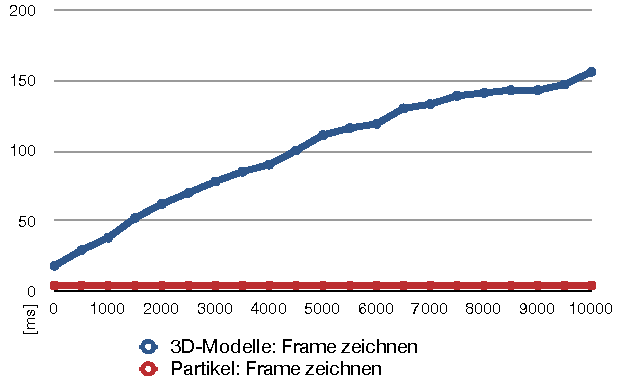
\includegraphics[width=\textwidth]{media/analysis3.pdf}
\caption{Dauer f�r das Zeichnen eines Frames in Millisekunden}
\label{analysis3}
\end{minipage}
\hspace{0.3cm}
\begin{minipage}[b]{0.48\linewidth}
\centering
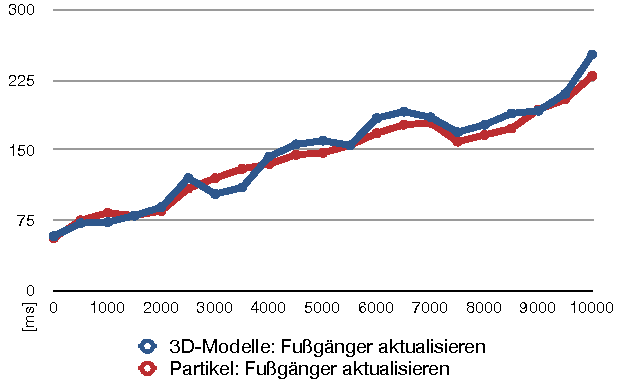
\includegraphics[width=\textwidth]{media/analysis2.pdf}
\caption{Dauer f�r das Aktualisieren der Fu�g�nger in Millisekunden}
\label{analysis2}
\end{minipage}
\end{figure}


Bei der Messung der JavaScript- und WebGL-Aufrufe lassen sich zwei Engstellen erkennen. Zum einen ist das die Berechnung der einzelnen Frames in der Grafikkarte, wie in Abbildung \ref{analysis3} dargestellt. Ausgef�hrt wird der Aufruf durch die Funktion \verb+requestAnimationFrame+ (vgl. Kapitel \ref{raf}). Bei Verwendung der 3D-Modelle steigt die Berechnungsdauer kontinuierlich mit der Zahl der Fu�g�nger an. Dagegen dauert das Zeichnen des Partikelsystems konstant etwa 4~ms, unabh�ngig von der Fu�g�ngeranzahl. Bei der Berechnungszeit eines Frames ist es irrelevant ob die Animation abgespielt wird oder nicht, da die Grafikkarte die Frames auch bei angehaltener Simulation berechnen muss.



W�hrend des Abspielens m�ssen zus�tzlich die Fu�g�ngerpositionen und -farben aktualisiert werden. Diese Berechnung stellt die zweite Engstelle dar. Unabh�ngig von der Berechnung der Frames wird alle 200~ms der n�chste Animationsschritt geladen. Die Aktualisierung muss per JavaScript im Prozessor erfolgen. Hier verhalten sich Partikelsystem und 3D-Modelle nahezu identisch, wie in Abbilung \ref{analysis2} zu erkennen ist. Die Ausf�hrungszeit bei der Darstellung der 3D-Modelle ist etwas h�her, da die Drehung der Figuren zus�tzlich berechenet werden muss. Ab etwa 9000 Objekten �berschreitet die Berechnungszeit die 200~ms und damit kann nicht mehr jeder einzelne Animationsschritt dargestellt werden.




\begin{wrapfigure}{r}{0.59\textwidth}
  %\begin{center}
    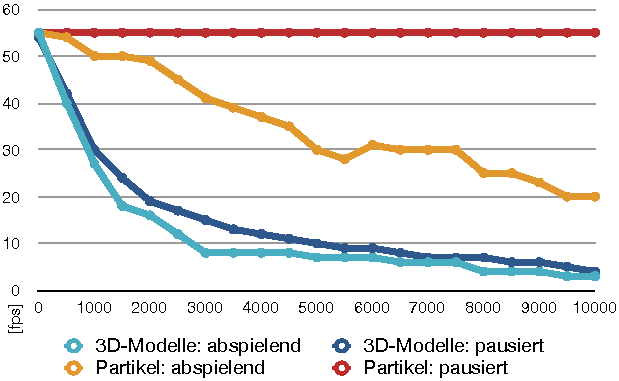
\includegraphics[width=0.6\textwidth]{media/analysis1.pdf}
  %\end{center}
  \caption{Vergleich der Framerate f�r Partikel und 3D-Modelle}
  \label{analysis1}
\end{wrapfigure}

Abschlie�end wurde die Framerate (engl. \emph{frames per second}, kurz \emph{fps}) analysiert. Dieser Wert gibt die Anzahl der Bilder an, die pro Sekunde in das canvas-Element gezeichnet werden und ist haupts�chlich abh�ngig von den Ausf�hrungszeiten der in Abbildung \ref{analysis3} und \ref{analysis2} betrachteten Funktionen. Welche Framerate f�r eine fl�ssige Animation notwendig ist unterscheidet sich im subjektiven Empfinden, sp�testens bei einer Framerate unter 20~fps ist jedoch ein deutliches Ruckeln bemerkbar. Ist die Animation pausiert, so m�ssen keine neuen Positionen der Fu�g�nger berechnet werden und es steht mehr Leistung f�r die Berechnung der Frames zur Verf�gung. Die Framerate bei der Verwendung des Partikelsystems ist im pausierten Zustand konstant bei 55~fps, w�hrend des Abspielens f�llt sie aber mit zunehmender Fu�g�ngerzahl. F�r die Gr��e des Testdatensatzes von etwa 10000 Fu�g�ngern ist eine fl�ssige Darstellung gerade noch m�glich. Bei der Verwendung der 3D-Modelle f�llt die Framerate deutlich schneller ab. Pausiert lassen sich etwa 2000 Fu�g�ngerobjekten mit 20~fps darstellen, l�uft die Animation sind ungef�hr 1500 Objekte bei gleicher Framerate m�glich. An dieser Stelle mangelt es an der Leistungsf�higkeit der Grafikkarte, mit schnelleren Grafikkarten w�ren mehr 3D-Modelle m�glich.

Die Darstellung als Partikelsystem ist f�r gro�e Datenmengen geeignet, da auch w�hrend dem Abspielen der Simulation noch eine akzeptable Framerate erreicht werden kann. F�r Standbilder und zur Analyse einzelner Zeitpunkte k�nnen trotzdem die 3D-Modelle verwendet werden. Ab 2000 Fu�g�ngern ist die Darstellung als Partikelsystem notwendig, bei Szenen mit mehr als 10000 Objekten war auf dem Testsystem keine fl�ssige Animation mehr m�glich.


% http://www.abendzeitung-muenchen.de/inhalt.simulation-wiesn-panik-diese-software-kann-sie-berechnen.2d7d8ded-1957-4507-b484-38a55c0651d9.html


\section{M�gliche Erweiterungen f�r SumoViz3D}
\label{erweiterungen}
Mit der Entwicklung von SumoViz3D wurde der Grundstein f�r eine vollwertige Visualisierung und Auswertung der Fu�g�ngersimulationsdaten gelegt. Eine gro�e Menge an Erweiterungsm�glichkeiten steht offen. Im Folgenden werden einige davon kurz erl�utert.

\begin{itemize}
\item Bisher ist die Darstellung verschiedener Stockwerke nicht m�glich. Diese Daten sind aber in der Ausgabedatei mit gespeichert und stehen somit zur Verf�gung. Gerade durch die dreidimensionale Darstellung in SumoViz3D w�rde es sich anbieten diese Funktionalit�t zu integrieren. Problematisch bei der Darstellung der Stockwerke ist die Verdeckung tieferliegenderer Stockwerke.

\item Aktuell ist es zwar m�glich, Standbilder der Visualisierung herunterzuladen, nicht aber den Ablauf der Animation in Form eines Videos. Die Standbildfunktion ist als Teil der canvas-API definiert und in der Funktion \verb+toDataURL()+ implementiert. Zwar ist es nicht m�glich Bewegtbilder direkt aus dem canvas-Element zu exportieren, aber �ber den Abruf aller Einzelbilder k�nnte ein Video generiert werden. Das Video m�sste entweder clientseitig berechnet, oder alle Einzelbilder an der Server �bertragen werden. Bei der clientseitigen Berechnung ist jedoch die Funktionalit�t mittels JavaScript sehr eingeschr�nkt.

\item Die Auswertung und Aufbereitung der Simulationsdaten l�sst sich noch wesentlich erweitern. Weitere Einf�rbungsoptionen f�r die Fu�g�nger beispielsweise nach Quelle oder Ziel sind denkbar. Entsprechende Daten sind nicht in den Datens�tzen enthalten und m�ssten berechnet werden. Denkbar sind auch statistische Auswertungswerkzeuge, um zum Beispiel den Fu�g�ngerdurchfluss an bestimmten Stellen zu messen.

\item Da durch die �nderung des Datenformats jeder Fu�g�nger nun einzeln identifizierbar ist, k�nnen diese Daten f�r die Visualisierung genutzt werden. Beispielsweise k�nnen die Wege der einzelnen Fu�g�nger mittels Linien dargestellt werden, die Kamera kann den Weg eines Fu�g�ngers verfolgen und zu jedem Fu�g�nger k�nnen Auswertungen der Geschwindigkeit und Dichte �ber die Zeit generiert werden.

\item Die einzelnen Zeitpunkte der Simulation werden in dieser Version von SumoViz3D schrittweise gerendert, wodurch die Fu�g�ngerobjekte von einer Position zur n�chsten springen. In einer Erweiterung k�nnte zwischen zwei aufeinanderfolgenden Schritten interpoliert und so ein fl�ssigerer Animationablauf erzeugt werden. Dazu muss das Zeichnen der Fu�g�nger in der \verb+requestAnimationFrame+-Methode stattfinden. In diesem Zuge kann auch eine Steuerung der Abspielgeschwindigkeit implementiert werden.

\item Die �bertragung der Simulationsdaten �ber das Internet kann, gerade bei umfangreichen Szenarien, einige Zeit in Anspruch nehmen. Hier k�nnten die Daten partiell bei Bedarf nachgeladen werden. Mit der Verwendung von JavaScript \emph{WebWorkern} w�re ein paralleles Herunterladen und parsen der kommenden Simulationsschritte m�glich, ohne den Ablauf der Visualisierung zu unterbrechen. Gr��e der Daten und Frequenz der Anfragen sollten abh�ngig von der Verbindungsqualit�t ermittelt und angepasst werden.
\end{itemize}


\section{Zusammenfassung}


Zusammenfassend l�sst sich sagen, dass die webbasierte Entwicklung von 3D-Applikationen noch in einer fr�hen Entwicklungsphase steckt. Sowohl bei der Implementierung der WebGL- und HTML5-Funktionen in den verschiedenen Browsern, als auch bei der verf�gbaren Rechenleistung ist in den n�chsten Jahren noch ein deutlicher Fortschritt zu erwarten. Auch die verwendete Grafikbibliothek THREE.js befindet sich ein stetiger Weiterentwicklung und wird in neueren Versionen noch effizienter und schneller werden.
Die SumoViz-Architektur, im speziellen die CouchDB-Datenbank, nutzt einen klassischen Trade-off der Informatik. Fehlende Rechenleistung wird durch einen Mehrverbrauch an Speicherplatz ausgeglichen. Die von CouchDB berechneten Daten werden gespeichert und m�ssen bei einem Aufruf nicht erneut berechnet werden. So kann die einmalige Berechnung der Daten l�ngere Zeit dauern, da die Daten danach sofort zur Verf�gung stehen. Zwar kostet dieses Verfahren viel Speicherplatz, aber nur so ist eine derartige Applikation mit den aktuellen Technologien �berhaupt realisierbar.
Trotzdem sind Webapplikationen eine gute M�glichkeit plattform�bergreifend Anwendungen zu entwickeln. Durch die Client-Server-Architektur stehen Daten �berall zur Verf�gung.
Vor einigen Jahren w�re eine dreidimensionale Simulationsvisualisierung im Browser noch komplett undenkbar gewesen. Mit SumoViz3D steht jetzt ein umfangreiches Werkzeug f�r die Darstellung und Analyse von Fu�g�ngerdaten zur Verf�gung. Damit kann es sowohl f�r die Forschung an neuen Modellen der Simulation als auch die Sicherheit auf Gro�veranstaltungen einen Beitrag leisten.




%�bernommen aus den Folien die als Hinweise zur Erstellung von Klausuren und �bungen existieren
%--------------------------- und auch schon Anhang und Literaturverzeichnis
\cleardoublepage
\begin{appendix}
% !TEX root = ../thesis.tex
%==============================================================================
% ATTACHMENT_A
\chapter{Beigef�gte CD}
\label{chap:bnhang}
%
%==============================================================================

Auf der beigef�gten CD befindet sich folgender Inhalt:
\begin{itemize}
	\item SumoViz3D Quellcode
	\item verschiedene Testdatens�tze (u.a. ``Betzenberg'', vgl. Kapitel \ref{betzenberg}) 
	\item MapReduce-Funktionen (vgl. Kapitel \ref{chapmapreduce})
	\item	diese Dokumentation, zusammen mit allen eingebundenen Grafiken
\end{itemize}


\end{appendix}
%\input{chapter/Appendix} %nur ein Beispiel
%---------------------------
\cleardoublepage
\listoffigures %Abbildungsverzeichnis
\listoftables %Tabellenverzeichnis
%---
\bibliographystyle{alpha}%{apalike}%{unsrt}{elsart-harv}
%\bibliography{./literature/references}%bei mehreren bib-files: \bibliography{bibfile1,bibfile2}
\begin{thebibliography}{99}


\bibitem[Kei10]{keith}
    \textbf{HTML5 for Web Designers} \\
    \textit{Jeremy Keith} \\
    A Book Apart, 2010

\bibitem[Pil10]{diveInto}
    \textbf{Dive into HTML5}  \\
    \textit{Mark Pilgrim}, 2010 \\

\bibitem[CB97]{vrml972}
    \textbf{The Annotated VRML 97 Reference Manual} \\
    \textit{Rikk Carey, Gavin Bell} \\
    Addison-Wesley Professional, 1997


\bibitem[Shr09]{Shreiner}
    \textbf{OpenGL Programming Guide} (Seventh Edition) \\
    \textit{Dave Shreiner} \\
    Addison-Wesley Longman, 2009

\bibitem[CJ12]{beginnersGuide}
    \textbf{WebGL Beginner's Guide}  \\
    \textit{Diego Cantor, Brandon Jones} \\
    Packt Publishing, 2012
    
\bibitem[Isi12]{Isi12}
    \textbf{SumoViz, HTML5-based Visualization of Pedestrian Simulation Data} \\
    \textit{Mustafa K. Isik} \\
    TU M�nchen, 10. Mai 2012

\bibitem[ALS10]{ALS10}
    \textbf{CouchDB: The Definitive Guide} \\
    \textit{J. Chris Anderson, Jan Lehnardt, Noah Slater} \\
    O'Reilly, 2010
    
\bibitem[Hol11]{Hol11}
    \textbf{Writing and Querying MapReduce Views in CouchDB} \\
    \textit{Bradley Holt} \\
    O'Reilly, 2011
    
\bibitem[McL11]{McL11}
    \textbf{What Is Node?} \\
    \textit{Brett McLaughlin} \\
    O'Reilly, 2011
    
\bibitem[Fla06]{Fla06}
    \textbf{JavaScript: The Definitive Guide} \\
    \textit{David Flanagan} \\
    O'Reilly, 2006
    
    
\cleardoublepage
\hspace{-\leftmargin}{\Large\bfseries Web-Referenzen} % W�ster Hack %-|



\bibitem[Tre11]{KhronosAbout}
    Neil Trevett: Building Markets for Advanced Devices through Open Standards \\
    \url{http://www.khronos.org/assets/uploads/developers/library/overview/khronos_overview.pdf}, abgerufen am 18.08.2012.

\bibitem[SGI]{SGI}
    SGI: OpenGL \\
    \url{http://www.sgi.com/products/software/opengl/?/overview.html}, \\ abgerufen am 18.08.2012.

\bibitem[Khr]{KhronosAbout2}
    About The Khronos Group \\
    \url{http://www.khronos.org/about}, abgerufen am 18.08.2012.

\bibitem[Goo]{devGoogle}
    Android Developers: Andriod 2.2 APIs \\
    \url{http://developer.android.com/about/versions/android-2.2.html}, \\ abgerufen am 18.08.2012.

\bibitem[App]{devApple}
    OpenGL ES for iOS \\
    \url{https://developer.apple.com/devcenter/ios/resources/opengl-es/}, \\ abgerufen am 18.08.2012.
    
\bibitem[Cab]{operawebgl}
    Luz Caballero (Opera): An introduction to WebGL \\
    \url{http://dev.opera.com/articles/view/an-introduction-to-webgl/}, \\ abgerufen am 18.08.2012.
        
\bibitem[Ope]{webgl}
    Khronos Group: WebGL - OpenGL ES 2.0 for the Web \\
    \url{https://www.khronos.org/webgl/}, abgerufen am 18.08.2012.
    
\bibitem[W3c]{W3Ccanvas}
    W3C: HTML5, The canvas element \\
    \url{http://www.w3.org/TR/html5/the-canvas-element.html#the-canvas-element}, \\ abgerufen am 18.08.2012.

\bibitem[WHc]{WHATWGcanvasContext}
    WHATWG: CanvasContexts \\
    \url{http://wiki.whatwg.org/wiki/CanvasContexts}, abgerufen am 18.08.2012.

\bibitem[Whc2]{WHATWGcanvas}
    WHATWG: The canvas element \\
    \url{http://www.whatwg.org/specs/web-apps/current-work/multipage/the-canvas-element.html}, abgerufen am 18.08.2012.

\bibitem[Sta1]{StatTop5Browser}
    StatCounter: Global Stats, Top 5 Browsers from Jun to Jul 2012 \\
    \url{http://gs.statcounter.com/#browser-ww-monthly-201206-201207-bar},  \\abgerufen am 18.08.2012.

\bibitem[MSFT]{MSWebGL}
    Microsoft Security Research \& Defense: WebGL Considered Harmful \\
    \url{http://blogs.technet.com/b/srd/archive/2011/06/16/webgl-considered-harmful.aspx}, abgerufen am 18.08.2012.

\bibitem[Sil]{Silverlight}
    Silverlight Blog: Silverlight 5 Available for Download Today \\
    \url{http://blogs.msdn.com/b/silverlight/archive/2011/12/09/silverlight-5-available-for-download-today.aspx}, abgerufen am 18.08.2012.

\bibitem[IEWeb]{IEWebGL}
    IEWebGL: WebGL for Internet Explorer \\
    \url{http://iewebgl.com}, abgerufen am 18.08.2012.

\bibitem[MDN]{MDNsop}
    Mozilla Developer Network: Same origin policy for JavaScript \\
    \url{https://developer.mozilla.org/en-US/docs/Same_origin_policy_for_JavaScript}, abgerufen am 18.08.2012.

\bibitem[W3cors]{cors}
    W3C: Cross-Origin Resource Sharing \\
    \url{http://www.w3.org/TR/cors/}, abgerufen am 18.08.2012.

\bibitem[AoGL]{iosopengl}
    OpenGL ES Programming Guide for iOS \\
    \url{http://developer.apple.com/library/ios/#documentation/3DDrawing/Conceptual/OpenGLES_ProgrammingGuide/Introduction/Introduction.html}, abgerufen am 19.08.2012.
    
\bibitem[SNE]{sonywebgl}
    Sony Ericsson Dev: WebGL \\
    \url{https://github.com/sonyericssondev/WebGL}, \\ abgerufen am 19.08.2012.
  
\bibitem[Sta2]{mobileos}
    StatCounter Global Stats: Top 8 Mobile Operating Systems from Jun to Jul 2012 \\
    \url{http://gs.statcounter.com/#mobile_os-ww-monthly-201206-201207-bar}, \\ abgerufen am 19.08.2012.

\bibitem[Con1]{contextwebgl}
    James Forshaw: WebGL -- A New Dimension for Browser Exploitation \\
    \url{http://www.contextis.com/research/blog/webgl/}, abgerufen am 19.08.2012.
    
\bibitem[Con2]{contextwebgl2}
    James Forshaw: WebGL -- More WebGL Security Flaws \\
    \url{http://www.contextis.com/research/blog/webgl/}, abgerufen am 19.08.2012.

\bibitem[Moz]{corsbug}
    Benoit Jacob: Cross-domain WebGL textures disabled in Firefox 5 \\
    \url{http://tinyurl.com/hacks-mozilla}, abgerufen am 19.08.2012.

\bibitem[Chr]{releaseChrome}
    Google Chrome Blog: A dash of speed, 3D and apps \\
    \url{http://chrome.blogspot.de/2011/02/dash-of-speed-3d-and-apps.html},  \\ abgerufen am 19.08.2012.

\bibitem[FF4]{releaseFirefox}
    Firefox 4 Release Notes \\
    \url{http://www.mozilla.org/en-US/firefox/4.0/releasenotes/}, \\ abgerufen am 19.08.2012.

\bibitem[Saf]{releaseSafari}
    WebGL Now Available in WebKit Nightlies \\
    \url{http://www.webkit.org/blog/603/webgl-now-available-in-webkit-nightlies/}, abgerufen am 19.08.2012.

\bibitem[Ope]{releaseOpera}
    Opera 12.00 for Windows Changelog \\
    \url{http://www.opera.com/docs/changelogs/windows/1200/}, abgerufen am 19.08.2012.

\bibitem[Sta3]{statVersion}
    StatCounter Global Stats: Top 12 Browser Versions from Jun to Jul 2012 \\
    \url{http://gs.statcounter.com/#browser_version-ww-monthly-201206-201207-bar}, abgerufen am 19.08.2012.

\bibitem[W3no]{nox3d}
    W3C HTML5: Things that you can't do with this specification because they are better handled using other technologies that are further described herein \\
    \url{http://www.w3.org/TR/html5/no.html}, abgerufen am 20.08.2012.    
    
\bibitem[W3a]{aboutw3c}
    W3C: �ber das W3C \\
    \url{http://www.w3.org/TR/html5/no.html}, abgerufen am 21.08.2012.
    
\bibitem[W3m]{w3cmembers}
    W3C: Current members \\
    \url{http://www.w3.org/Consortium/Member/List}, abgerufen am 21.08.2012.
    
\bibitem[MDN1]{mozdom}
    Mozilla Developer Network: What is the DOM? \\
    \url{https://developer.mozilla.org/en-US/docs/Gecko_DOM_Reference/Introduction}, abgerufen am 21.08.2012.
    
\bibitem[HTML]{html5rocks} HTML5 Rocks: WebGL Fundamentals \\
    \url{http://www.html5rocks.com/en/tutorials/webgl/webgl_fundamentals/}, \\ abgerufen am 20.8.2012

\bibitem[THREE]{threejsdocs}
    THREE.js r50 Dokumentation \\
    \url{http://mrdoob.github.com/three.js/docs/50/}, abgerufen am 21.08.2012

\bibitem[X3D]{x3dom}
    X3DOM: About \\
    \url{http://www.x3dom.org/?page_id=2}, abgerufen am 21.08.2012

\bibitem[Web3]{x3domhtml}
    X3D and HTML5 \\
    \url{http://www.web3d.org/x3d/wiki/index.php/X3D_and_HTML5}, \\ abgerufen am 21.08.2012

\bibitem[VRML1]{vrml10}
    The Virtual Reality Modeling Language: Version 1.0 Specification \\
    \url{http://www.web3d.org/x3d/specifications/vrml/VRML1.0/}, \\ abgerufen am 21.08.2012

\bibitem[VRML97]{vrml97}
    The Virtual Reality Modeling Language: International Standard  \\
    \url{http://www.web3d.org/x3d/specifications/vrml/ISO-IEC-14772-VRML97//}, \\ abgerufen am 21.08.2012

\bibitem[2Dc]{2dcontext}
    W3C: HTML Canvas 2D Context \\
    \url{http://www.w3.org/TR/2dcontext/}, abgerufen am 21.08.2012

\bibitem[spec]{specGraph}
    Peter Kr�ner: HTML5 Spezifikations-�bersicht \\
    \url{https://github.com/SirPepe/SpecGraph}, abgerufen am 22.08.2012

\bibitem[W3l]{w3cpr}
    W3C: W3C Confirms May 2011 for HTML5 Last Call \\
    \url{http://www.w3.org/2011/02/htmlwg-pr.html }, abgerufen am 22.08.2012

\bibitem[VRML1a]{vrml10}
    The Virtual Reality Modeling Language: Version 1.0 Specification \\
    \url{http://www.web3d.org/x3d/specifications/vrml/VRML1.0/}, \\ abgerufen am 22.08.2012

\bibitem[VRMLa]{vrml97}
    The Virtual Reality Modeling Language: International Standard \\
    \url{http://www.web3d.org/x3d/specifications/vrml/ISO-IEC-14772-VRML97//},  \\ abgerufen am 22.08.2012

\bibitem[W32d]{2dcontext}
    W3C: HTML Canvas 2D Context \\
    \url{http://www.w3.org/TR/2dcontext/}, abgerufen am 22.08.2012

\bibitem[Win]{windows}
    Microsoft: Timeout Detection and Recovery of GPUs \\
    \url{http://msdn.microsoft.com/en-us/windows/hardware/gg487368.aspx}, \\ abgerufen am 28.08.2012

\bibitem[KhrSec]{KhrSec}
    Khronos Group: WebGL Security \\
    \url{http://msdn.microsoft.com/en-us/windows/hardware/gg487368.aspx}, \\ abgerufen am 28.08.2012

\bibitem[SPON1]{spon1}
    Spiegel Online: Warum die Wege des Menschen unberechenbar sind \\
    \url{http://spon.de/ac51E}, abgerufen am 01.09.2012

\bibitem[SPON2]{spon2}
    Spiegel Online: Der k�rzeste Weg ist das Ziel \\
    \url{http://spon.de/adlhZ}, abgerufen am 01.09.2012

\bibitem[jQu]{jQu}
    jQuery UI \\
    \url{http://jqueryui.com/home}, abgerufen am 03.09.2012

\bibitem[MrD]{MrD}
    THREE.js Stats - JavaScript Performance Monitor \\
    \url{https://github.com/mrdoob/stats.js}, abgerufen am 01.09.2012
    
\bibitem[COL]{COL}
    COLLADA Digital Asset and FX Exchange Schema \\
    \url{https://collada.org/mediawiki/index.php/COLLADA_-_Digital_Asset_and_FX_Exchange_Schema}, abgerufen am 05.09.2012

\bibitem[W3s]{W3s}
    W3C: WebStorage \\
    \url{http://www.w3.org/TR/webstorage/}, abgerufen am 06.09.2012
    
\bibitem[Res12]{Res12}
    John Resig: How JavaScript Timers Work \\
    \url{http://ejohn.org/blog/how-javascript-timers-work/}, abgerufen am 06.09.2012
    
\bibitem[Iri11]{Iri11}
    Paul Irish: requestAnimationFrame for smart animating \\
    \url{http://paulirish.com/2011/requestanimationframe-for-smart-animating/}, \\ abgerufen am 07.09.2012
    
\bibitem[Gub09]{Gub09}
    Martin Gubisch: Kugelkoordinaten \\
    \url{http://www.martingubisch.de/cms/upload/files/tutorien/09\%20Kugelkoordinaten.pdf}, abgerufen am 07.09.2012
        
\bibitem[MSDN]{MSDN}
    Microsoft: Billboarding \\ 
    \url{http://msdn.microsoft.com/de-de/library/bb172358(VS.85).aspx}, \\ abgerufen am 07.09.2012

\bibitem[vdB00]{vdB00}
    John van der Burg: Building an Advanced Particle System \\
    \url{http://www.gamasutra.com/view/feature/3157/building_an_advanced_particle_.php}, abgerufen am 07.09.2012
    
\bibitem[Wie]{Wie}
    Lyle Wiedeman: Information on the HSV color space \\
    \url{http://dcssrv1.oit.uci.edu/~wiedeman/cspace/me/infohsv.html}, \\ abgerufen am 07.09.2012
    
\end{thebibliography}



%---
\end{document}
